\documentclass[
11pt, % The default document font size, options: 10pt, 11pt, 12pt
%oneside, % Two side (alternating margins) for binding by default, uncomment to switch to one side
english, % ngerman for German
singlespacing, % Single line spacing, alternatives: onehalfspacing or doublespacing
%draft, % Uncomment to enable draft mode (no pictures, no links, overfull hboxes indicated)
%nolistspacing, % If the document is onehalfspacing or doublespacing, uncomment this to set spacing in lists to single
%liststotoc, % Uncomment to add the list of figures/tables/etc to the table of contents
%toctotoc, % Uncomment to add the main table of contents to the table of contents
%parskip, % Uncomment to add space between paragraphs
%nohyperref, % Uncomment to not load the hyperref package
headsepline, % Uncomment to get a line under the header
%chapterinoneline, % Uncomment to place the chapter title next to the number on one line
%consistentlayout, % Uncomment to change the layout of the declaration, abstract and acknowledgements pages to match the default layout
]{MastersDoctoralThesis} % The class file specifying the document structure

\usepackage[utf8]{inputenc} % Required for inputting international characters
\usepackage[T1]{fontenc} % Output font encoding for international characters
\usepackage{mathpazo} % Use the Palatino font by default
\usepackage{algorithm}
\usepackage[noend]{algpseudocode}
\usepackage[]{graphicx}
\usepackage[backend=biber,natbib=true]{biblatex}
\addbibresource{biblio.bib}
\usepackage[autostyle=true]{csquotes} % Required to generate language-dependent quotes in the bibliography

%----------------------------------------------------------------------------------------
%	MARGIN SETTINGS
%----------------------------------------------------------------------------------------

\geometry{
	paper=a4paper, % Change to letterpaper for US letter
	inner=2.5cm, % Inner margin
	outer=3.8cm, % Outer margin
	bindingoffset=.5cm, % Binding offset
	top=1.5cm, % Top margin
	bottom=1.5cm, % Bottom margin
	%showframe, % Uncomment to show how the type block is set on the page
}

%----------------------------------------------------------------------------------------
%	THESIS INFORMATION
%----------------------------------------------------------------------------------------

\thesistitle{Thesis Title} % Your thesis title, this is used in the title and abstract, print it elsewhere with \ttitle
\supervisor{Dr. Davide \textsc{Rossini}} % Your supervisor's name, this is used in the title page, print it elsewhere with \supname
\examiner{} % Your examiner's name, this is not currently used anywhere in the template, print it elsewhere with \examname
\degree{Master degree} % Your degree name, this is used in the title page and abstract, print it elsewhere with \degreename
\author{Francesca \textsc{Collu}} % Your name, this is used in the title page and abstract, print it elsewhere with \authorname
\addresses{} % Your address, this is not currently used anywhere in the template, print it elsewhere with \addressname

\subject{Physics} % Your subject area, this is not currently used anywhere in the template, print it elsewhere with \subjectname
\keywords{} % Keywords for your thesis, this is not currently used anywhere in the template, print it elsewhere with \keywordnames
\university{\href{http://www.university.com}{University of Pisa}}
%
\includegraphics[]{marchio_unipi_black.eps} % Your university's name and URL, this is used in the title page and abstract, print it elsewhere with \univname
\department{\href{http://department.university.com}{Department or School Name}} % Your department's name and URL, this is used in the title page and abstract, print it elsewhere with \deptname
\group{\href{http://researchgroup.university.com}{Research Group Name}} % Your research group's name and URL, this is used in the title page, print it elsewhere with \groupname
\faculty{\href{http://faculty.university.com}{Faculty Name}} % Your faculty's name and URL, this is used in the title page and abstract, print it elsewhere with \facname

\AtBeginDocument{
\hypersetup{pdftitle=\ttitle} % Set the PDF's title to your title
\hypersetup{pdfauthor=\authorname} % Set the PDF's author to your name
\hypersetup{pdfkeywords=\keywordnames} % Set the PDF's keywords to your keywords
}

\begin{document}

\frontmatter % Use roman page numbering style (i, ii, iii, iv...) for the pre-content pages

\pagestyle{plain} % Default to the plain heading style until the thesis style is called for the body content

%----------------------------------------------------------------------------------------
%	TITLE PAGE
%----------------------------------------------------------------------------------------

\begin{titlepage}
\begin{center}

\vspace*{.06\textheight}
{\scshape\LARGE \univname\par}\vspace{1.5cm} % University name
\textsc{\Large Master Thesis}\\[0.5cm] % Thesis type

\HRule \\[0.4cm] % Horizontal line
{\huge \bfseries \ttitle\par}\vspace{0.4cm} % Thesis title
\HRule \\[1.5cm] % Horizontal line
 
\begin{minipage}[t]{0.4\textwidth}
\begin{flushleft} \large
\emph{Author:}\\
\href{http://www.johnsmith.com}{\authorname} % Author name - remove the \href bracket to remove the link
\end{flushleft}
\end{minipage}
\begin{minipage}[t]{0.4\textwidth}
\begin{flushright} \large
\emph{Supervisor:} \\
\href{http://www.jamessmith.com}{\supname} % Supervisor name - remove the \href bracket to remove the link  
\end{flushright}
\end{minipage}\\[3cm]
 
\vfill

\large \textit{A thesis submitted in fulfillment of the requirements\\ for the degree of \degreename}\\[0.3cm] % University requirement text
\textit{in the}\\[0.4cm]
\groupname\\\deptname\\[2cm] % Research group name and department name
 
\vfill

{\large \today}\\[4cm] % Date
%\includegraphics{Logo} % University/department logo - uncomment to place it
 
\vfill
\end{center}
\end{titlepage}

%----------------------------------------------------------------------------------------
%	QUOTATION PAGE
%----------------------------------------------------------------------------------------

% \vspace*{0.2\textheight}

% \noindent\enquote{\itshape {Interrogare il passato non serve a niente. È al futuro che bisogna fare le domande. Senza futuro, il presente è solo disordine.}}\bigbreak

% \hfill J.C.Izzo, \emph{Chourmo}

%----------------------------------------------------------------------------------------
%	ABSTRACT PAGE
%----------------------------------------------------------------------------------------

% \begin{abstract}
% \addchaptertocentry{\abstractname} % Add the abstract to the table of contents
% The Thesis Abstract is written here (and usually kept to just this page). The page is kept centered vertically so can expand into the blank space above the title too\ldots
% \end{abstract}

%----------------------------------------------------------------------------------------
%	LIST OF CONTENTS/FIGURES/TABLES PAGES
%----------------------------------------------------------------------------------------

\tableofcontents % Prints the main table of contents

%\listoffigures % Prints the list of figures

%\listoftables % Prints the list of tables

%----------------------------------------------------------------------------------------
%	ABBREVIATIONS
%----------------------------------------------------------------------------------------

% \begin{abbreviations}{ll} % Include a list of abbreviations (a table of two columns)

% \textbf{LAH} & \textbf{L}ist \textbf{A}bbreviations \textbf{H}ere\\
% \textbf{WSF} & \textbf{W}hat (it) \textbf{S}tands \textbf{F}or\\

% \end{abbreviations}

%----------------------------------------------------------------------------------------
%	PHYSICAL CONSTANTS/OTHER DEFINITIONS
%----------------------------------------------------------------------------------------

%\begin{constants}{lr@{${}={}$}l} % The list of physical constants is a three column table

% The \SI{}{} command is provided by the siunitx package, see its documentation for instructions on how to use it

%Speed of Light & $c_{0}$ & \SI{2.99792458e8}{\meter\per\second} (exact)\\
%Constant Name & $Symbol$ & $Constant Value$ with units\\

%\end{constants}

%----------------------------------------------------------------------------------------
%	SYMBOLS
%----------------------------------------------------------------------------------------

%\begin{symbols}{lll} % Include a list of Symbols (a three column table)

%$a$ & distance & \si{\meter} \\
%$P$ & power & \si{\watt} (\si{\joule\per\second}) \\
%Symbol & Name & Unit \\

%\addlinespace % Gap to separate the Roman symbols from the Greek

%$\omega$ & angular frequency & \si{\radian} \\

%\end{symbols}

%----------------------------------------------------------------------------------------
%	DEDICATION
%----------------------------------------------------------------------------------------

%\dedicatory{To my lovely parents.} 

%----------------------------------------------------------------------------------------
%	THESIS CONTENT - CHAPTERS
%----------------------------------------------------------------------------------------

\mainmatter % Begin numeric (1,2,3...) page numbering

\pagestyle{thesis} % Return the page headers back to the "thesis" style

\chapter*{Introduction}
\addcontentsline{toc}{chapter}{Introduction}

\label{Introduction}

Open quantum systems are physical systems coupled with an environment with which they exchange information. Studying the dynamics of open systems is not an easy problem, due to the complexity of the interaction between the parts involved. In order to overcome this difficulty, over the decades several analytical e numerical methods have been developed. In addition to these more "traditional" approaches, over the last decades have been investigated and advanced the field of quantum simulators: experimental platforms that reproduce Hamiltonian models analyzable with difficulty. Their advantage is the fact that the quantum simulators are quantum systems that can be insulated from the environment or with parameters easily tunable in order to replicate the model under consideration.

  
\chapter{Open Quantum Systems}
\label{Chapter1}

% Define some commands to keep the formatting separated from the content 
\newcommand{\keyword}[1]{\textbf{#1}}
\newcommand{\tabhead}[1]{\textbf{#1}}
\newcommand{\code}[1]{\texttt{#1}}
\newcommand{\file}[1]{\texttt{\bfseries#1}}
\newcommand{\option}[1]{\texttt{\itshape#1}}

%----------------------------------------------------------------------------------------
The world we live in is constituted by parts that communicate with each other and exchange information \textcolor{red}{[EXAMPLES]}. The difficulty of describing it, lies in the complexity of the interactions between those parts. To overcome these problems, simplifications and mathematical representation have been brought about in this field: in the following we will see some of them. 

Several resources have been helpful in the \dots

\section{Closed and Open Quantum Systems}
Before we explore the field of open quantum systems, let us observe what are the differences between a closed and an open quantum system and why different approaches are required to treat these two distinct kinds of system. First of all, let us define a \emph{closed} system as a physical system which does not exchange any information with its surroundings. On the contrary, an \emph{open} system is a physical system that interacts with the environment in which it is. 

In this section, we will briefly look at the different approaches in the study of the dynamics in closed and open quantum systems. 

\subsection{Pure and mixed states: the density matrix formalism}
First of all, it is useful consider another formalism in addition to that used normally for handling pure states, i.e. states that can be described by a single wave function. We now introduce the \emph{density matrix} formalism for managing the so-called mixed states, although - as we will see - it can be used also for pure states.

Quantum systems prepared in such a way that their state vector being obtained performing a \emph{maximal measurement}, in the sense that the maximum possible information has been acquired (all values of a complete set of commuting observables have been ascertained), are in a pure state. 

Quantum systems for which the maximum possible information is not available, are said to be in mixed state and are called \emph{statistical mixtures}.

Let us consider a system consisting of an ensemble of N sub-systems $\alpha = 1, 2, \dots , N$. We suppose that every sub-system is in a pure state $\ket{\psi_\alpha}$. Then, we choose a complete set of basis vectors $\ket{n}$, such that $\sum_n \ket{n}\bra{n} = \mathds{1}$. Let us expand the pure states in the basis $\{\ket{n}\}$:
\begin{equation*}
    \ket{\psi_\alpha} = \sum_n c_n^{\alpha}\ket{n},
\end{equation*}
where the coefficients $c_n^{(\alpha)}$ are such that
\begin{equation*}
    \sum_n |c_n^{(\alpha)}|^2 = 1.
\end{equation*}
Now let us consider an observable represented by an operator $A$; its expectation value in the pure state $\psi_\alpha$ is:
\begin{align}
    \braket{A}_\alpha &= \bra{\psi_\alpha}A\ket{\psi_\alpha} \\
                      \label{braket_A}
                      &= \sum_n \sum_{n'} c_{n'}^{(\alpha)*} c_n^{(\alpha)} \bra{n'}A\ket{n} \\
                      &= \sum_n \sum_{n'} \braket{n|\psi_\alpha}\braket{\psi_\alpha|n'} \bra{n'}A\ket{n}.
\end{align}
The average value of A over the ensemble is
\begin{equation}
\label{stat_averageA}
    \braket{A} = \sum_{\alpha = 1}^N w_\alpha \langle A \rangle_\alpha,
\end{equation}
where the coefficients $w_\alpha$ are the statistical weight of the pure states $\ket{\psi_\alpha}$, i.e. the probability of finding the system in this state. 
So the $w_\alpha$ are such that
\begin{equation}
\label{charact_weights}
    0 \leq w_\alpha \leq 1
\end{equation}
and 
\begin{equation*}
    \sum_{\alpha=1}^N w_\alpha = 1.
\end{equation*}
Using the result~\ref{braket_A} in the~\ref{stat_averageA}, we obtain:
\begin{align}
    \braket{A} &= \sum_{\alpha = 1}^N \sum_n \sum_{n'} w_\alpha c_{n'}^{(\alpha)*} c_n^{(\alpha)} \bra{n'}A\ket{n} \\
                \label{total_stat_average}
               &= \sum_{\alpha = 1}^N \sum_n \sum_{n'} \braket{n|\psi_\alpha}w_\alpha \braket{\psi_\alpha|n'} \bra{n'}A\ket{n}.
\end{align}
We now introduce the \emph{density operator}
\begin{equation}
    \rho = \sum_{\alpha = 1}^N \ket{\psi_\alpha} w_\alpha \bra{\psi_\alpha},
\end{equation}
whose representation in the basis $\{n\}$ gives us the density matrix:
\begin{equation}
    \rho_{nn'} = \bra{n}\rho\ket{n'} = \sum_{\alpha = 1}^N w_\alpha c_{n'}^{(\alpha)*} c_n^{(\alpha)}.
\end{equation}
So, returning to the~\ref{total_stat_average} in the definition of the density matrix, we observe that:
\begin{equation*}
    \braket{A} = \sum_n \sum_{n'} \bra{n}\rho\ket{n'}\bra{n'}A\ket{n} = \Tr({\rho A}).
\end{equation*}
It is worth stressing the fact that the knowledge of the density matrix enables us to obtain the ensemble average of A.

Anyway, this leads us to the first of the three fundamental characteristics of the density matrix, that is:
\begin{equation}
    \Tr(\rho) = 1,
\end{equation}
that is true if we make the assumption that the $\ket{\psi_\alpha}$ are normalized to unity. If they are not, then the ensemble average of A is given by
\begin{equation}
    \braket{A} = \frac{\Tr(\rho A)}{\Tr(\rho)}.
\end{equation}
The second characteristic of the density matrix is that it is Hermitian, namely
\begin{equation}
    \bra{n}\rho\ket{n'} = \bra{n'}\rho\ket{n}^*.
\end{equation}
The third characteristic arises from the observation of the diagonal elements of $\rho$:
\begin{equation}
    \rho_{nn} = \bra{n}\rho\ket{n} = \sum_{\alpha = 1}^N w_\alpha |c_{n}^{(\alpha)}|^2,
\end{equation}
which tells us, with the~\ref{charact_weights}, that
\begin{equation}
    \rho_{nn} \geq 0,
\end{equation}
i.e. $\rho$ is a positive semi-definite matrix.
It is worth stress the physical interpretation of the diagonal elements; $w_\alpha$ is the probability of finding the system in the pure state $\psi_\alpha$, while $|c_{n}^{(\alpha)}|^2$ is the probability of finding $\psi_\alpha$ in the state $\ket{n}$. So, $\rho_{nn}$ gives the probability of finding a member of the ensemble in the state $\ket{n}$.

\subsection{Closed Quantum Systems}
\label{closed_systems}
Quantum mechanics establishes that the time evolution of a state vector $\ket{\psi(t)}$ is predicted by the Schrödinger equation:
\begin{equation}
\label{eqn:schrod_eq}
    i\frac{d}{dt}\ket{\psi(t)} = H(t)\ket{\psi(t)},
\end{equation}
where $H(t)$ is the Hamiltonian of the closed system and Planck's constant $\hbar$ has been set equal to 1.
The solution of this equation can be written in terms of the unitary time-evolution operator $U(t, t_0)$:
\begin{equation}
\label{eqn:schrod_u}
    \ket{\psi(t)} = U(t, t_0)\ket{\psi(t_0)},
\end{equation}
where $t_0 < t$. If we substitute the equation~\ref{eqn:schrod_u} into the~\ref{eqn:schrod_eq}, we obtain:
\begin{equation}
    i\frac{d}{dt}U(t, t_0) = H(t)U(t, t_0),
\end{equation}
subject to the initial condition
\begin{equation}
    U(t_0, t_0) = \mathds{1}.
\end{equation}
We can write the dynamics of a closed system using the density matrix formalism seen in the previous section. In order to do this, let us assume that at a initial time $t_0$ the state of the system is characterized by the density matrix
\begin{equation*}
    \rho(t_0) = \sum_{\alpha = 1}^N w_\alpha \ket{\psi_\alpha(t_0)} \bra{\psi_\alpha(t_0)},
\end{equation*}
that at a time $t$ evolves in this way:
\begin{equation*}
    \rho(t) = \sum_{\alpha = 1}^N w_\alpha U(t,t_0)\ket{\psi_\alpha(t_0)} \bra{\psi_\alpha(t_0)}U(t,t_0)^\dagger,
\end{equation*}
that is
\begin{equation*}
     \rho(t) = U(t,t_0) \rho(t_0) U(t,t_0)^\dagger.
\end{equation*}
Differentiating with respect to time the last equation we have
\begin{equation}
\label{eqn:motion_closed_dm}
    \frac{d}{dt}\rho(t) = -i[H(t), \rho(t)]
\end{equation}
i.e. an equation of motion for the density matrix, often called the \emph{Liouville-von Neumann equation}.


\subsection{Open Quantum Systems}
Now we can go into a more specific definition of open quantum systems. It can be defined as a system $S$ coupled with another quantum system $B$, called the \emph{environment}. Usually, the total system $S+B$ is treated as a closed system, so it follows Hamiltonian dynamics. The interactions between the two sub-systems cause an evolution in the state of the open system $S$, which can no longer be represented by unitary, Hamiltonian dynamics. Following the definitions given in~\cite{pet_breuer:open_quantum}, an environment with an infinite number of degrees of freedom such that the frequencies of the modes form a continuum, is called \emph{reservoir}. Also, when the reservoir is in thermal equilibrium state, is called \emph{bath}.

Let us call $\mathcal{H}_S$ and $\mathcal{H}_B$ the Hilbert spaces of the system and the environment, respectively. The Hilbert space of the combined system is given by the tensor product $\mathcal{H}_{S+B} = \mathcal{H}_S \otimes \mathcal{H}_B$. So, the total Hamiltonian can be written in this way:
\begin{equation}
    H(t) = H_S \otimes \mathds{1}_B + \mathds{1}_S \otimes H_B + H_I(t),
\end{equation}
where $H_S$ and $H_B$ are the free Hamiltonians of the system and the environment, respectively, and $H_I(t)$ is the Hamiltonian describing the interactions between $S$ and $B$.

At this point, we must find a relation between the density matrix $\rho \in \mathcal{H}$ and $\rho_S \in \mathcal{H}_S$; it is given by the partial trace over the environment $B$\textcolor{red}{[PROOF?]}:
\begin{equation}
    \rho_S = \Tr_B(\rho).
\end{equation}
This can help us in the study of the dynamics of the so-called \emph{reduced} density matrix $\rho_S$. Indeed, we can write:
\begin{equation}
    \rho_S(t) = \Tr_B\{\rho(t)\};
\end{equation}
observing that we assumed the total system to be \emph{closed}, it evolves unitarily so we have:
\begin{equation}
    \rho_S(t) = \Tr_B\{U(t, t_0)\rho(t_0)U(t, t_0)^\dagger\},
\end{equation}
where $U(t, t_0)$ is the time-evolution operator of the combined system $S+B$. So we can use the equation of motion~\ref{eqn:motion_closed_dm} and trace over the degrees of freedom of the environment, in order to obtain the equation of motion for the $\rho_S(t)$:
\begin{equation}
    \frac{d}{dt}\rho_S(t) = -i \Tr_B[H(t), \rho(t)].
\end{equation}

\section{Approximate Dynamics of Open Quantum Systems}

\subsection{The Dynamical Map}
\subsection{The Lindblad Master Equation}
\section{Many-Body Open Quantum Systems}
%One of the main goals in scientific research is coming up to quantum simulation; this is due to the fact that in several physical fields there are mechanisms that cannot be simulated by classical computers: the essential aim is using a controlled quantum device to investigate another quantum system. Experiments have shown that superconducting circuits are able to manipulate and measure at the level of a few qubits and microwave photons, as a quantum simulator~\cite{Nat.Phys2012}. They can be treated as open systems because of the loss of photons, coupled to the feeding in additional photons through continuous external driving. Moreover, they are greatly flexible, because of their nanofabricated nature and almost every parameter involved is widely tunable. In~\cite{PhysRevX.7.011016}, it has been demonstrated that QED cavity lattices act as a controllable platform guiding understanding of non-equilibrium physics. 

\chapter{Quantum Simulators of Open Many-Body Systems}
\label{chapter2}
\epigraph{Can a quantum system be probabilistically simulated by a classical universal computer? [\dots] \\The answer is certainly, no!}{\textit{Richard P. Feynman}}

Open quantum many-body systems represent a challenging area of study, due to the exponential growth of the number of freedom degrees with respect to the number of the constituent particles. The scientific community has built many strategies to overcome this obstacle, by developing and refining several analytical and numerical methods. In addition to these, another approach was proposed, based on the use of quantum simulators~\cite{quantum_sim_feynman}.

In the present chapter we report a review of some of the most relevant ideas in the field of quantum simulators; in particular, the last section focuses on the simulation of spin systems, of remarkable interest in view of the model studied in this work.

%\section{Basics of Dynamics}
%As expressed in the previous chapter, an open quantum system can be described in terms of %$\rho_S$, the reduced matrix given by averaging over the environment: 
%\begin{equation}
%    \rho_S = \Tr_E(\rho).
%\end{equation}
%Under certain conditions discussed in section~\ref{appr_dynam_oqs}, the evolution of %$\rho_S$ is delineated by the Lindblad master equation:
%\begin{equation}
%\label{eqn:lindbladME_manyBody}
%    \dot{\rho_S} = -i[H_{sys}, \rho_S] - \sum_{a=1}^{N^2-1} %\gamma_a\mathcal{D}[L_a]\rho_S,
%\end{equation}
%where the first term expresses the usual unitary evolution under the system Hamiltonian %$H_sys$ and the second term represents the influence of the environment over the system %through the dissipation rate $\gamma_a$ and the dissipators
%\begin{equation*}
%    \mathcal{D}[L_a]\rho_S \equiv \frac{1}{2} \Bigl( [L_a\rho_S, L_a^{\dagger}] + [L_a, %\rho_S L_a^{\dagger}] \Bigl).
%\end{equation*}
%The Linblad operators determine the nature of the decoherence process, e.g. photon loss %($a$), qubit relaxation ($\sigma^-$), qubit dephasing ($\sigma^z$), and so on.
%The steady-state solution can be found rewriting this equation in terms of a linear %algebra problem. First of all, the Hilbert space for a system consisting of N spins, has %an orthonormal Fock-state basis such as $\ket{\phi_1, \phi_2, \dots \phi_N}$.
%For solving the equation
%\begin{equation*}
%    \dot{\rho}_S = 0,
%\end{equation*}
%outlining a \emph{superoperator formalism}~\cite{davRoss_wordpress} is advantageous. 
%Every linear operator $\hat{A}$ acting on the Hilbert space $\mathcal{H}$ can be associated with a vector in a superoperator space:
%\begin{equation*}
%    \hat{A} = \sum_{ij} A_{ij} \ket{i}\bra{j} \quad \rightarrow \quad |A\rangle\rangle = \sum_{ij} A_{ij} \ket{i}\ket{j}.
%\end{equation*}
%This way, the density operator can be vectorized and re-arranged as a \emph{super-ket} $|\rho_S\rangle\rangle$ with $N^2$ components, allowing eq.~\ref{eqn:lindbladME_manyBody} to be formally rewritten in terms of the Liouvillian superoperator. Thus, the steady-state equation can be read as an eigenvalue equation:
%\begin{equation}
%\label{eqn:SS_masterEq}
%    \hat{L}|\rho_S\rangle\rangle = 0.
%\end{equation}
%Its solution can be obtained computing the eigenvector of the $N^2 \times N^2$ super-operator $\hat{L}$ corresponding to the null eigenvalue.

%It is important to stress that the number of elements of the matricial representation of the superoperator grows with $N^4$. So, straightforward brute-force integration methods become unfeasible even for small system sizes.

\section{Quantum Many-Body Systems}
\label{hubb_model}
Quantum many-body systems are systems made up by a certain number of interacting particles. Typical quantum many-body systems are represented by Hubbard-like models or spin chains. 
A prototype of these systems is described by the non-dissipative Bose-Hubbard model~\cite{Greiner_bose_hubbard}: an interacting boson gas in a lattice potential. The Hamiltonian reads:
\begin{equation}
    H = -J\sum_{\langle i,j \rangle} a^{\dagger}_i a_j + \sum_i \epsilon_i n_i+ \frac{1}{2} U \sum_i n_i(n_i -1 ),
\end{equation}
where the notation $\langle i, j \rangle$ denotes the sum over nearest-neighbour sites; $a_i$ and $a^{\dagger}_i$ are the bosonic creation and annihilation operators respectively, on the i-th site; they obey the bosonic commutation relations:
\begin{equation}
    [a_i, a_j^\dagger] = \delta_{ij}, \quad [a_i, a_j] = 0 = [a_i^\dagger, a_j^\dagger].
\end{equation}

$n_i$ is the number operator, which counts the number of bosons in the i-th site; $\epsilon_i$ is the energy due to the external harmonic confinement to which the bosons are undergone. The $J$ term is the one responsible for the hopping between adjacent sites due to the tunnel coupling; it is the matrix element:
\begin{equation}
    J = -\int d^3x \quad w(\Vec{x}-\Vec{x_i})(-\frac{\nabla^2}{2m}+V(\Vec{x}))w(\Vec{x}-\Vec{x_j}),
\end{equation}
where $w(\Vec{x}-\Vec{x_i})$ is a single particle Wannier function localized to the i-th site, $V(\Vec{x})$ is the lattice potential and $m$ is the mass of a single boson.
$U$ is instead the matrix element for the interaction between bosons in the same site; it is:
\begin{equation}
    U = \frac{4\pi a}{m} \int d^3x \quad |w(\Vec{x})|^4, 
\end{equation}
$a$ being the scattering length. 

If the tunnel coupling term $J$ dominates the hamiltonian $(J \gg U)$, the ground-state energy is minimized if the single-particle wavefunctions of the $N$ bosons is spread out over the entire $M$ sites of the lattice; so the many-body ground state reads:
\begin{equation}
    \ket{\Psi_{SF}} \propto \Bigl( \sum_{i=1}^M a^{\dagger}_i \Bigl)^N \ket{0},
\end{equation}
i.e. all bosons occupy the same extended Bloch state. As pointed out by~\cite{Greiner_bose_hubbard}, an important feature of this state is that the probability distribution of the occupation $n_i$ of bosons on a single site is Poissonian, so that its variance is given by $\langle n_i \rangle$; this means that it is well described by a macroscopic wavefunction with long-range phase coherence throughout the lattice.

If the on-site interaction term $U$ dominates $(U \gg J)$, the ground state of the system will instead consist of localized wavefunctions with a fixed number of bosons per site that minimized the energy; the many-body ground state will be a product of local Fock states for each site:
\begin{equation}
    \ket{\Psi_{MI}} \propto \prod_{i=1}^M \Bigl( a^{\dagger}_i\Bigl)^N \ket{0}.
\end{equation}

The two kinds of ground state have been labeled with the subscripts "SF" and "MI", specifying the two phases to which the system may be found: superfluid and Mott insulator phases.


\section{Quantum Simulators: Controllable Many-Body Systems}
In order to overcome the difficulty in studying open many-body systems, over the years several analytical and numerical methods have been developed. In addition to these more "traditional" approaches, during the last twenty years it arose the idea of studying a quantum system by using a properly designed quantum device. The essential aim of this new strategy lies in the employment of controlled quantum devices called \emph{quantum simulators}; they are systems able to experimentally emulate the Hamiltonian model bearing the non-trivial properties of the system under study. The usefulness of this approach is twofold~\cite{Tomadin_Fazio}:  not only it allows to explore properties of the model in regions that are elusive to the analytical and numerical studies, but also it consents to test to which limits the Hamiltonian model is appropriate to describe the system or whether additional ingredients are required.

Since the Josephson junction arrays~\cite{josephsonArrays}, that were probably the first quantum simulators in the history of modern physics, much progress has been made especially with the advent of cold atoms in optical lattices.

\subsection{Cold Atoms in Optical Lattices}
\begin{figure}
    \centering
    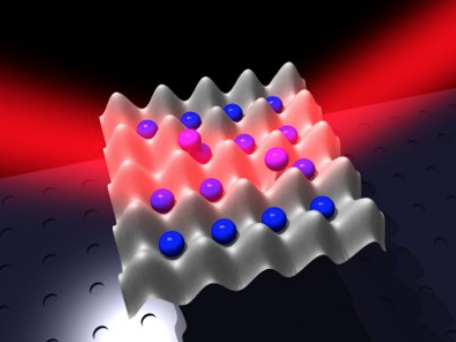
\includegraphics[scale=0.7]{Figures/optical_lattice.png}
    \captionsetup{width=1.\linewidth}
    \caption{Optical lattices are crystals made of light: lasers beams interfere to form a periodic potential in which ultracold atoms are trapped. Figure taken from from the LENS laboratory webpage, Florence~\cite{LENS_Florence}.}
    \label{fig:optical_lattice}
\end{figure}

The employment of cold atoms in optical lattices has proved to be a successful way to create simulators of a large variety of strongly interacting systems~\cite{ultracoldAtoms_condMatter}. 

In short, optical lattices are created by making laser beams counter-propagating interfere with each other~\cite{optical_lattice_interview}. The result is a standing wave with a periodic pattern (see sketch in fig.~\ref{fig:optical_lattice}). Then, ultracold atoms can be trapped in the potential wells, creating first a Bose-Einstein condensate or a cold gas of fermionic atoms and then slowly ramping up the laser beams to create the periodic lattice potential. 

Ultracold atoms in optical lattices represent nearly perfect realization of fermionic and bosonic Hubbard models\footnote{The (fermionic) Hubbard model in one dimension is characterized by the following Hamiltonian:
\begin{equation*}
    H = -t\sum_{\langle ij \rangle}c^{\dagger}_{i\sigma}c_{j\sigma} + U\sum_i n_{i\uparrow}n_{i\downarrow},
\end{equation*}
where $c_i$ and $c^{\dagger}_i$ are the fermionic creation and annihilation operators respectively, on the i-th site; they obey the fermionic commutation relations:
\begin{equation*}
    \{c_i, c_j^\dagger\} = \delta_{ij}, \quad \{c_i, c_j\} = 0 = \{c_i^\dagger, c_j^\dagger\}.
\end{equation*}
The first term in $H$ represents the hopping between adjacent sites and the second represents the on-site interaction between particles. The $n_{i\sigma}$ are the occupation numbers, that count the number of electron with spin $\sigma$ in site $i$. This model is very similar to that described in section~\ref{hubb_model}, with the difference of nature of particles considered: here they are fermions, in Bose-Hubbard model are bosons instead. 
In the text, the plural \emph{Hubbard models} refers to the several variations of this model.
}~\cite{ultracoldAtoms_condMatter} and they are usually employed to simulate non-dissipative systems. However, new efforts have been made in order to introduce dissipation in these devices. 
In fig.~\ref{fig:optical_lattice_dissipation}, a sketch of the implementation of the effective dissipative process in an optical \emph{superlattice} is shown. The so-called superlattice is made up coupling driven-dissipative ultracold atoms in an optical lattice with a coherently driven reservoir. 

\begin{figure}[H]
    \centering
    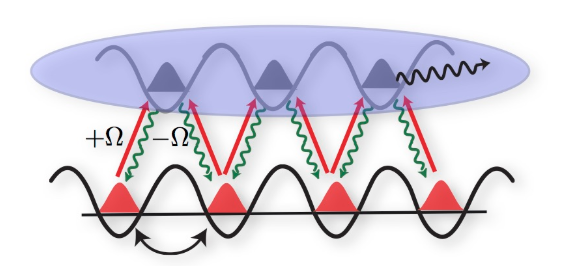
\includegraphics[scale=0.7]{Figures/optical_lattice_dissipation.png}
    \captionsetup{width=1.\linewidth}
    \caption{Schematic realization of the effective dissipative process with ultracold atoms in an optical superlattice. Figure taken from~\cite{diehl_wEbsite}.}
    \label{fig:optical_lattice_dissipation}
\end{figure}

An interesting study over the possibility of using cold atoms to simulate dissipative many-body systems, has been done by~\cite{BEC_dissipativeMBsimulator}. The authors of this work discuss the example of a driven dissipative Bose-Einstein condensate of bosons, where atoms in optical lattice are coupled to a bath of Bogoliubov excitations; the atomic current represents local dissipation. It was assumed that the atoms can be described by a Bose-Hubbard model, having the following Hamiltonian:
\begin{equation}
    H = H_0 + V \equiv -J \sum_{\langle i,j \rangle} a_i^{\dagger} a_j + \frac{1}{2}U \sum_i a_i^{\dagger 2} a_j^2,
\end{equation}
where $H_0$ represents the kinetic energy of bosons hopping between
adjacent lattice sites with amplitude $J$, $V$ is the onsite interaction
with strength $U$ and $a_i$ ($a_i^{\dagger}$) are bosonic destruction (creation)
operators for atoms at i-th site. At this point, an appropriate choice of jump operators allows to couple the system to a bath so that it is driven to a pure many-body state by quasi-local dissipation. Applying standard linearization schemes in the weakly interacting situations led to obtain the solution of the master equation~\ref{eqn:lindblad_eqn}. The steady-state solution seems to have properties similar to those of bosons in thermal contact to a heat bath.

Another strategy involves trapping Rydberg atoms in optical lattices. Rydberg atoms are alkali-like atoms with a single electron promoted into a highly excited orbital~\cite{carusotto_ciuti}. The presence of these atoms enhances photon-photon interaction; the presence of a single photon in the system is able to drive away from resonance condition all atoms contained in a surrounding volume. If the optical density is sufficiently high, a second photon travelling across this volume can be absorbed or suffer a phase shift; this can be use to obtain an effective blockade effect.

\subsection{QED-Cavity Arrays}
In the last few decades the field of quantum simulators has been enriched by a new idea, based on arrays of QED cavities~\cite{Tomadin_Fazio} (sketched in fig.~\ref{fig:QED_cavities}), in which light resonates and interacts with matter contained therein.  A compelling aspect of this kind of devices is the competition between two phenomena: while on the one hand light-matter interaction inside the cavity leads to photon blockade, on the other hand photon hopping between neighbouring cavities favors delocalization.

\begin{figure}
    \centering
    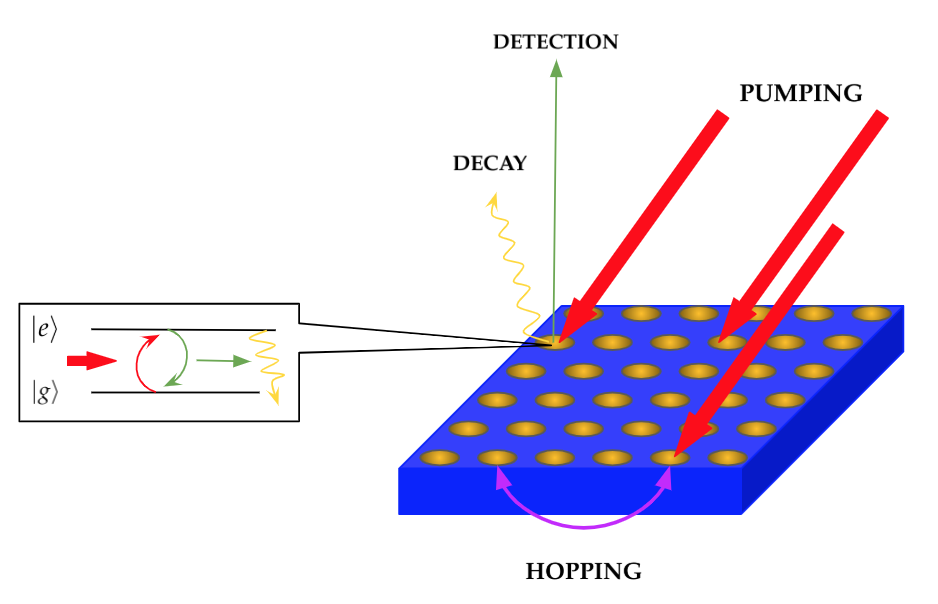
\includegraphics[scale=0.7]{Figures/QED_cavity.png}
    \captionsetup{width=1.\linewidth}
    \caption{Sketch of array of QED cavities. In the inset there is a draft of the interaction between the two-level system and the photon resonating in the cavity and then decaying. Photons in the cavities have finite life-time, so there is a coherent external drive.}
    \label{fig:QED_cavities}
\end{figure}

QED cavities are mathematically described by the Jaynes-Cummings model~\cite{shore_knight}, in which one mode of the cavity interacts with a two-level system. By ignoring light-matter interaction, a single cavity confines several modes of electromagnetic field and each of them is quantized as a harmonic oscillator. If one considers a cavity with a single mode with frequency $\omega$, the Hamiltonian describing such a system can be written as
\begin{equation}
\label{eqn:single_cavity}
    H = \omega a^{\dagger}_la_l,
\end{equation}
where $a_l (a_l^{\dagger})$ annihilates (creates) a quantum of light in the mode of the l-th cavity.
An array of cavities sufficiently close to allow for photon hopping, can be described by eq.~\ref{eqn:single_cavity} to which the following term should be added:
\begin{equation}
    H_{\text{hop}} = -J (a^{\dagger}_la_{l+1} + h.c.),
\end{equation}
where $J$ is associated with the tunneling rate.
Now, if the light-matter interaction is introduced, the Hamiltonian can be written in this way:
\begin{equation}
    H = \sum_l H_l^{(0)} - J \sum_{\langle l, l' \rangle}(a^{\dagger}_la_{l'} + h.c.),
\end{equation}
where the term $H_l^{(0)}$ describes the light-matter interaction. In particular, we want to study QED cavities so the Hamiltonian term $H_l^{(0)}$ is the Jaynes-Cummings model:
\begin{equation}
\label{eqn:Jaynes-Cummings}
    H_{l,\text{JC}}^{(0)} = \varepsilon \sigma^z_l + \omega a^{\dagger}_la_l + g(\sigma^+_l a_l + \sigma^-_l a_l^{\dagger}),
\end{equation}
where $\sigma^\pm_l$ are the raising/lowering operators for the two-level system and $\varepsilon$ indicates the transition energy between the two levels.
The spectrum of the Hamiltonian~\ref{eqn:Jaynes-Cummings} is anharmonic, meaning the presence of the two-level system induces a repulsion between the photons in the cavity, so that in the cavity only a photon can be present at the same time. Qualitatively, this can be explained by the fact that a single photon in the cavity modifies the effective resonance frequency, so that the injection of another photon is inhibited. This nonlinear process is known as \emph{photon blockade} and has been named in analogy with the Coulomb blockade effect of electron transport through mesoscopic devices.
% QED cavities
    % sketch of QED cavities
    % optical cavities: photon blockade effect
    % Jaynes-Cummings nonlinearities
% pag. 55 Carusotto-Ciuti
% fig.10 di Noh2016

An array of cavities in the impenetrable photon regime has been theoretically studied~\cite{carusotto_ciuti}. As sketched in fig.~\ref{fig:cavities_ring}, a continuous pumping is considered. The transmission and/or absorption spectrum of the system shows the Tonks-Girardeau nature of the steady-state of photon gas, i.e. the fermionization of photons.

\begin{figure}
    \centering
    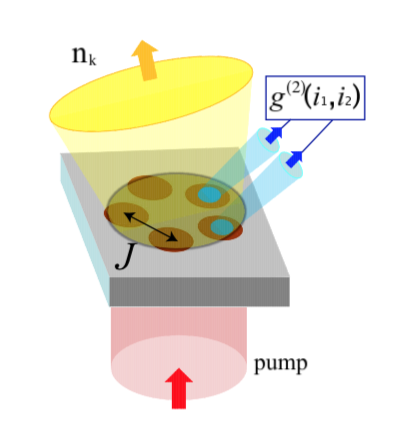
\includegraphics[scale=0.7]{Figures/cavities_ring.png}
    \captionsetup{width=1.\linewidth}
    \caption{Sketch of an array of five cavities arranged in a ring geometry with periodic boundary conditions; the system is driven by a laser. Figure taken from~\cite{carusotto_ciuti}.}
    \label{fig:cavities_ring}
\end{figure}

% pag.5 Tomadin-Fazio per optical lattices vs cavity arrays

\subsection{Superconducting Circuits}
As for QED-cavities, also for superconducting circuits, or QED-circuits, light-matter interaction is central. In these simulators~\cite{supercircuitsQED}, the quantum "particles" are excitations, not physical particles subjected to conservation laws, so they naturally access non-equilibrium physics. Photonic modes can be realized with on-chip microwave resonators, typically Fabry-Perot kind of cavities. A qubit coupled to such a resonator can be described by the Jaynes-Cummings model:
\begin{equation}
    H_{\text{JC}} = \omega_r a^{\dagger}a+ \varepsilon\sigma^+\sigma^- + g(a\sigma^+ + a^{\dagger}\sigma^-),
\end{equation}
where $\omega_r$ and $\varepsilon$ are the the photon and qubit excitation frequencies, and $a^{\dagger}$, a, $\sigma^+$ and $\sigma^-$ denote the corresponding raising and lowering operators. An example of these devices can be seen in fig.~\ref{fig:superconducting_circuits}.

\begin{figure}
    \centering
    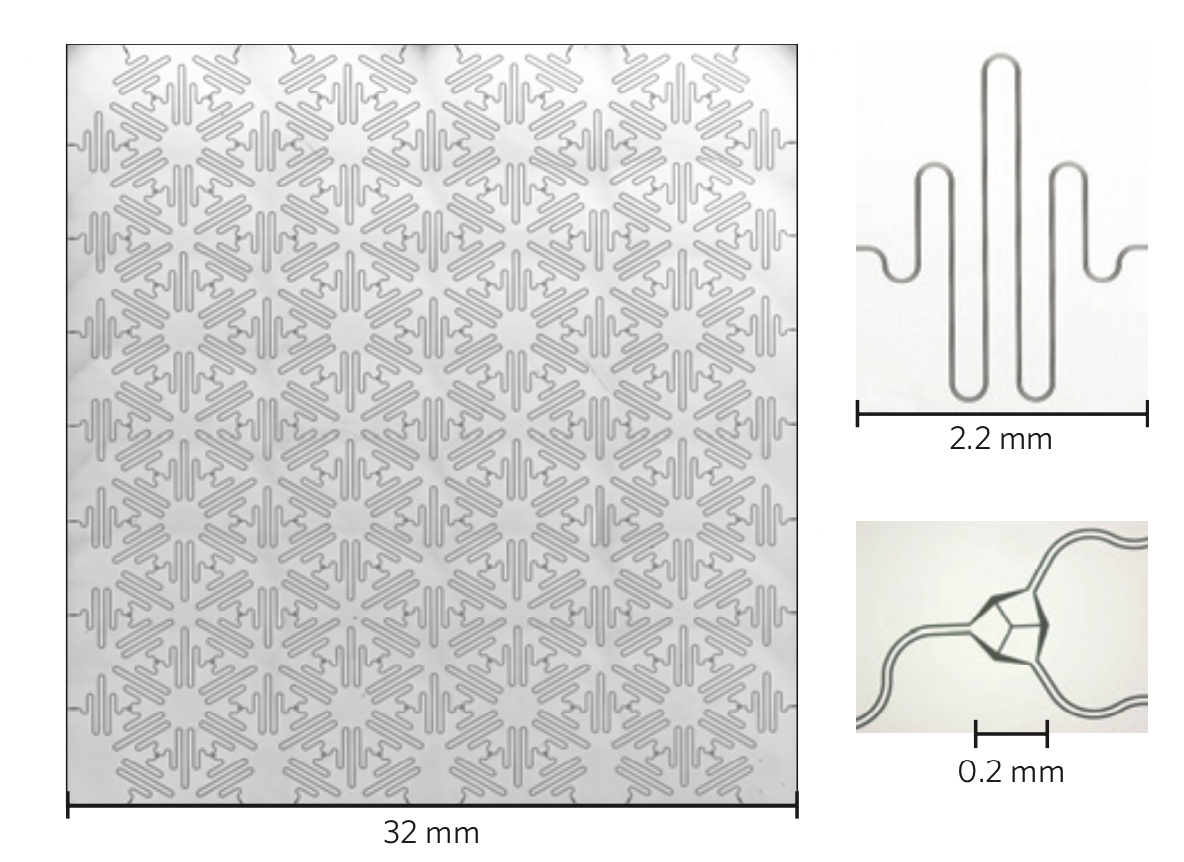
\includegraphics[scale=0.6]{Figures/superconducting_circuits.png}
    \captionsetup{width=1.\linewidth}
    \caption{Example of an array of resonators forming a honeycomb pattern. On the left, more than two hundred microwave cavities are coupled in a Kagome lattice, a natural two-dimensional lattice. Each cavity is coupled to two neighbours, through a capacitor that enables photon hopping. On the bottom-right, it can be seen the simmetric three-way capacitor that ensures uniform hopping rates throughout the array. Figure taken from~\cite{supercircuitsQED}.}
    \label{fig:superconducting_circuits}
\end{figure}

\subsection{Arrays of Optomechanical Systems}
A recent proposal by~\cite{optomechanical_arrays} considers making arrays of optomechanical systems. The essential idea is that at each site of such an array, a localized mechanical mode interacts with an optical mode of a cavity driven by laser beams; the interaction occurs via radiation pressure. This way, both photons and phonons can hop between neighbouring sites. Because of the experimental complexity of this kind of device, only a single cavity has been cooled to the ground state~\cite{Lee_Haffner_Cross}, so far. 

The work of~\cite{optomechanical_arrays} focuses on the transition of the collective mechanical motion from an incoherent state (due to quantum noise) to an ordered state with phase-coherent mechanical oscillations; for this dynamics, the dissipative effects induced by the optical modes play a crucial role. Indeed, they allow the mechanical modes to have self-induced oscillations, once the optomechanical amplification rate exceeds the intrinsic mechanical damping; on the other hand, the quantum noise prevents the mechanical modes from synchronizing.


\section{Quantum Simulation of Spin Systems}
Interacting two level systems, either spins or qubits, are of central importance in Quantum Information and Condensed Matter Physics. 
%\textcolor{red}{In magnetic compounds where spin lattices appear naturally the addressability of individual spins is unfortunately extremely hard to achieve because the spatial separation between neighboring spins is very small and the timescales of interesting processes can be very short.}

Since the discover of the \emph{photon blockade}~\cite{ph_blockade}, it has been realized that the cavity mode is well described by a spin-$1/2$ Hamiltonian. Few years later, the Jaynes-Cummings model in the Mott regime was shown to simulate a XY spin model~\cite{angelakis}. In particular, the studied system consisted of coupled electromagnetic cavities doped with a single two-level system; it has been shown that it is possible to observe an insulator phase of total (atomic plus photonic, i.e. \emph{polaritonic}) excitations. From such a system, an effective XY Hamiltonian arises, with spin up (down) corresponding to the presence (absence) of a polariton.

A scheme for realizing the Ising spin-spin interaction has been proposed in~\cite{LiGuGong}, with a system consisting in trapped two-level atoms in one dimensional coupled microcavities. 

A more complicated system has been investigated in~\cite{Hartmann_XYZ}, which uses three-level atoms in micro-cavities coupled to each other via the exchange of virtual photons; it is shown that it can model an anisotropic Heisenberg spin-1/2 chain in an external magnetic field. The two spin polarizations $\ket{\uparrow}$ and $\ket{\downarrow}$ are represented by two long-lived atomic levels of a $\Lambda$ level-structure; let us see why. The quantized mode of the cavity together with external lasers can induce a Raman transition between these two lowest-lying states.  With appropriately chosen detunings, the dominant Raman transition between the two lowest-lying states involves one laser and one cavity photon. This implies that the emission and absorption of virtual photons in the cavity is confined to only two states per atom, the long-lived ones, so that it can be described by a spin-1/2 Hamiltonian. The coupling of virtual photons between neighbouring cavities simulates $\sigma^x\sigma^x$ and $\sigma^y\sigma^y$ interactions; the effective spin can be coupled to an effective magnetic field $\sigma^z$; using the same atomic level configuration but a different set-up of the external sources an effective $\sigma^z\sigma^z$ interaction is obtained.

\begin{figure}[H]
    \centering
    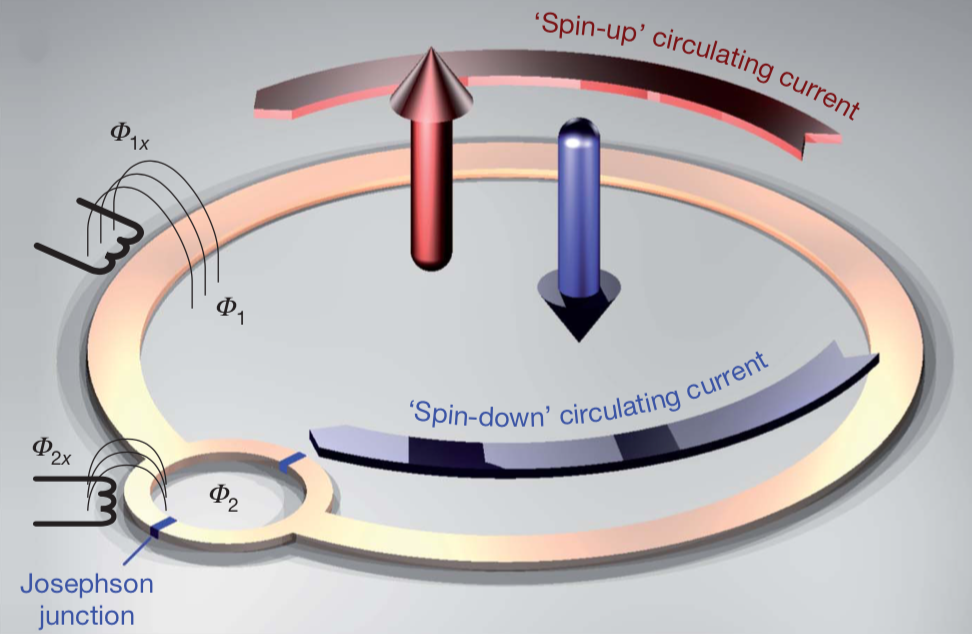
\includegraphics[scale=0.5]{Figures/superconductinCircuit_SpinSystem.png}
    \captionsetup{width=1.\linewidth}
    \caption{Simplified schematic of a superconducting flux qubit \\acting as a quantum mechanical spin~\cite{8spinChain_simulatedByQubits}.}
    \label{fig:superconductinCircuit_SpinSystem}
\end{figure}

It has been possible using superconducting circuits to simulate small spin chains, by directly coupling a number of superconducting qubits~\cite{8spinChain_simulatedByQubits}. Fig.\ref{fig:superconductinCircuit_SpinSystem} shows two superconducting loops in the qubit, each subject to an external flux bias $\Phi_{1x}$ and $\Phi_{2x}$. The dynamics of the device can be modelled as a quantum mechanical double-well potential. The two lowest energy states of the system correspond to clockwise or anticlockwise circulating current in loop 1. Considering only these two states (in the limit of low temperature it is a valid approximation), the qubit dynamics is that of an Ising spin. Qubits are then coupled together using programmable coupling elements; this allows to tune the spin coupling in a continous way between ferromagnetic and antiferromagnetic character. The behaviour of this system is well described by an Ising model Hamiltonian:
\begin{equation}
    H = \sum_{i=1}^{N} h_i\sigma_i^z + \sum_{i,j=1}^{N} J_{ij}\sigma_i^z\sigma_j^z.
\end{equation}
In this way, it has been possible to simulate a one-dimensional 8-sites spin chain, with the ends polarized in opposite directions.
\chapter{Numerical Methods for Open Quantum Systems}
\label{chapter3}
\epigraph{Hilbert space is a big place.}{\textit{Carlton Caves}}
As we have seen in the previous chapter, the study of an open quantum system requires the knowledge of its density matrix, solution of the Lindblad master equation~\cite{presk:quant_info}:
\begin{equation*}
    \dot{\rho} = \mathcal{L}[\rho],
\end{equation*}
where
\begin{equation}
\label{eqn:lindblad_eqn}
    \mathcal{L}[\rho] \equiv -i[H, \rho] - \sum_{a=1}^{N^2-1}\gamma_a\Bigl(\frac{1}{2}L_a^{\dagger}L_a\rho + \frac{1}{2}\rho L_a^{\dagger}L_a - L_a\rho L_a^{\dagger}\Bigl),
\end{equation}
$N$ being the dimension of Hilbert space.

In such a system the number of variables scales as the square of the dimension of the Hilbert space; for example, in a spin-$\frac{1}{2}$ system made up by $n$ elements, the size of the Hilbert space $\mathcal{H}$ is $2^n$ while the \emph{liouvillian dimension} equals to $2^{2n} \times 2^{2n}$. Clearly, a direct integration of the equation~\ref{eqn:lindblad_eqn} can be made only for systems with a very limited number of elements. One only needs to note the fact that for a brute-force integration of the equation~\ref{eqn:lindblad_eqn} for a system consisting of $8$ sites, about $34$ GB of memory would be necessary\footnote{This calculation considers the fact that the liouvillian contains, in general, complex numbers, each of them valued with a single precision (32 bit).}.

Nevertheless, some techniques for exact diagonalization of Liouvillian superoperator~\ref{eqn:lindblad_eqn} has been developed. To name but one, that devised by Prosen in ref.~\cite{Prosen_2008} for studying a quadratic system of interacting fermions coupled to a set of Markovian baths, prescribes to express the~\ref{eqn:lindblad_eqn} in terms of anticommuting super-operators which act on the Fock space of density operators. 
%The numerical methods employed in open quantum system problems can be classified in those that have a wave-function approach (quantum trajectories method, mean field method) and those that decompose the system into blocks (corner-space renormalization method, matrix product density operators method).

However, as seen previously, a direct integration of master equation for an open many-body system becomes unfeasible even for relatively small sizes, so conceiving numerical strategies seems to be necessary.

One of them is based on the \emph{mean field} approach; the essential idea is considering the mean value of the Hamiltonian and, as suggested by Gutzwiller, factorizing the density matrix, defining a mean field density matrix $\rho_{MF} = \prod_j\rho_j$, where $\rho_j$ is the single site density matrix. In this way, all correlations and interactions between sites are neglected, so we can say it is a crude approximation for an interacting many-body system. In order to (partially) overcome this problem, the \emph{cluster mean field} method was developed: in this method a set of contiguous sites are isolated from the rest of the system. As explained in~\cite{PhysRevX.6.031011}, this method suggests to write the Hamiltonian as $H_{CMF} = H_\mathcal{C} + H_{\mathcal{B(C)}}$, where the first term describes the exact interactions inside the cluster while the second term represents the mean-field interactions between the cluster and the sites on its boundary $\mathcal{B(C)}$. The global density matrix will be $\rho_{CMF} = \bigotimes \rho_\mathcal{C}$, where the $\rho_\mathcal{C}$ is the density matrix of the $\mathcal{C}$th cluster. One should note that, when the cluster is made up by a single site, the method becomes the above-mentioned standard one. 

Others important numerical methods are the ones essentially based on the \emph{linked cluster expansions}~\cite{oitmaa}, in which the quantities of interest are expressed as sums of contributions from a sequence of clusters of sites; in particular, only connected clusters contribute. In~\cite{PhysRevX.6.021037} an application of this idea to the Liouvillian is done.

In this section, we will examine some of the numerical techniques used for studying open quantum systems with very different approaches.

Two of the three numerical methods analyzed in this chapter are essentially based on the Wilson's \emph{renormalization group} approach~\cite{RevModPhys.47.773} combined with the fundamental contribution of the White's \emph{density matrix renormalization group} (DMRG) method~\cite{s_white:dmrg} and are the \emph{corner-space renormalization} and the \emph{matrix product density operators} methods. They both use the idea of a system decomposition into blocks; even if the basic idea is the same, the developed approaches are actually different.

The first numerical method analyzed in the section~\ref{chapt2_qtm} is the \emph{quantum trajectories} method, based on the evolution of a Monte Carlo wave function.

%%%%%%%%%%%%%%%%%%%%%%%%%%%%%%%%%%%%%%%%%%%%%%%%%%%%%%%%%%%%%%%%%%%
%%%%%%%%%%%%%%%%%%%%%%%%%%%%%%%%%%%%%%%%%%%%%%%%%%%%%%%%%%%%%%%%%%%
%%%%%%%%%%%%%%%%%%%%%%%%%%%%%%%%%%%%%%%%%%%%%%%%%%%%%%%%%%%%%%%%%%%
\section{The Quantum Trajectories (QT) Method}
\label{chapt2_qtm}
The \emph{quantum trajectories method} is an estabilished numerical method, in which pure states are the subjects of the study, instead of density matrices. This means that, if the Hilbert space has dimension $N$, the number of involved parameters ($\sim N$) is much smaller than the one required in calculations with density matrices ($\sim N^2$). This method was originally proposed in 1992 by Dalibard, Castin and Mølmer in~\cite{PhysRevLett.68.580}, then generalized in~\cite{Molmer:93}, as a stochastic unraveling of the master equation, namely a stochastic evolution for the wave function of a system coupled to a reservoir. It has been proved~\cite{PhysRevLett.68.580, Molmer:93} the equivalence of this \emph{Monte Carlo wave-function} approach with the master equation treatment.

The idea of this method can be summarised in the following way.

First of all, given the~\ref{eqn:lindblad_eqn}, let us note that the first three terms of this equation can be regarded as the evolution performed by an effective non-Hermitian Hamiltonian, that is~\cite{PhysRevA.69.062317}:
\begin{equation*}
    H_{\text{eff}} = H_s + \text{i}K,
\end{equation*}
with
\begin{equation*}
    K = -\frac{1}{2}\sum_\mu L_{\mu}^{\dagger}L_{\mu}.
\end{equation*}
Indeed, we see that:
\begin{equation*}
    -\text{i}[H_\text{eff}, \rho] = -\text{i}[H_s, \rho] - \frac{1}{2}\sum_\mu \{L_{\mu}^{\dagger}L_{\mu}, \rho\}.
\end{equation*}

The \textbf{last term} of the~\ref{eqn:lindblad_eqn}, is the one responsible for the so-called \emph{quantum jumps}; for this reason, the representation under which we have written the~\ref{eqn:lindblad_eqn} is called \emph{quantum jump picture}~\cite{PhysRevA.69.062317}. 

At an initial time $t_0$, the density matrix of the system is in a pure state
\[
\rho(t_0) = \ket{\phi(t_0)}\bra{\phi(t_0)};
\]
after a time $dt$, it evolves to the following statistical mixture:
\begin{equation}
    \rho(t_0 + dt) = \Bigl(1-\sum_\mu dp_\mu \Bigl)\ket{\phi_0}\bra{\phi_0} + \sum_\mu dp_\mu \ket{\phi_\mu}\bra{\phi_\mu},
\end{equation}
where
\begin{equation}
    dp_\mu = \bra{\phi(t_0)}L_{\mu}^{\dagger}L_{\mu}\ket{\phi(t_0)}dt
\end{equation}
is the probability that a jump occurs; in this case, the system evolves in the state
\begin{equation}
\label{eqn:phi_mu}
    \ket{\phi_\mu} = \frac{L_\mu}{\abs{L_\mu\ket{\phi(t_0)}}}\ket{\phi(t_0)}.
\end{equation}
Otherwise, if no jump happens, the system evolves according to the effective Hamiltonian $H_{eff}$ in the following way:
\begin{equation}
    \ket{\phi_0} = \frac{(1-\textrm{i}H_{eff}dt)}{\sqrt{1-\sum_\mu dp_\mu}}\ket{\phi(t_0)}.
\end{equation}

In order to decide if the jump occurs or not, a Monte Carlo method will be integrated in this picture. Namely, an uniform distribution in the unit interval $[0,1]$ is taken under consideration; for every experiment, a pseudo-random number $\epsilon$ is chosen from this uniform distribution, i.e. a coin is tossed: depending on the result of the throw, the possible situations are the following:
\begin{itemize}
    \item if $\epsilon < \sum_\mu dp_\mu$, the system jumps to one of the states $\ket{\phi_\mu}$, defined in~\ref{eqn:phi_mu}. In particular:
    \begin{itemize}
        \item if $0 \leq \epsilon \leq dp_1$, the system jumps to $\ket{\phi_1}$;
        \item if $dp_1 < \epsilon \leq dp_2$, the system jumps to $\ket{\phi_2}$;
        \item and so on;
    \end{itemize}
    \item if $\epsilon > \sum_\mu dp_\mu$, the system evolves to the state $\ket{\phi_0}$.
\end{itemize}

This process has to be repeated as many times as $n = \frac{T}{dt}$, where $T$ is the whole elapsed time during the evolution. Let us note that $dt$ must be taken much smaller than the scales relevant for the evolution of the system.

Every \emph{experiment}, i.e. every throw of the coin, gives a different \emph{quantum trajectory}, which can be used to calculate the mean value of an observable $A$ at a certain time $t$, in this way:
\begin{equation}
    \langle A(t)\rangle = \bra{\phi_i(t)}A\ket{\phi_i(t)}.
\end{equation}
Since this results from a Monte Carlo process, we can consider the mean value over $N$ \emph{experiments}:
\begin{equation}
    \langle A(t)\rangle = \lim_{N\to\infty} \frac{1}{N}\sum_{i=1}^{N}\bra{\phi_i(t)}A\ket{\phi_i(t)}.
\end{equation}
So, to sum up we can say a few things about QT algorithm; it allows to do the so-called \emph{stochastic unraveling} of the master equation, using pure states instead of density matrices: as we have seen, this simplifies the computational complexity of the problem. However, this method has an important limit: it does not prevent the exponential growth respect to the size of the system. Trying to work this out will be a task of the methods that will be analyzed in the next two sections.

%%%%%%%%%%%%%%%%%%%%%%%%%%%%%%%%%%%%%%%%%%%%%%%%%%%%%%%%%%%%%%%%%%%
%%%%%%%%%%%%%%%%%%%%%%%%%%%%%%%%%%%%%%%%%%%%%%%%%%%%%%%%%%%%%%%%%%%
%%%%%%%%%%%%%%%%%%%%%%%%%%%%%%%%%%%%%%%%%%%%%%%%%%%%%%%%%%%%%%%%%%%
\section{The Corner-Space Renormalization (CSR) Method}
\label{chapter3_csr}
The numerical methods based on renormalization group à la Wilson present a computational problem due to the increase of the dimensions of the Hilbert space, while the blocks are merged; the fundamental aim of the corner-space renormalization (CSR) method~\cite{PhysRevLett.115.080604} is to deal with this problem and try to overcome the limitation mentioned above. 


\begin{figure}[H]
    \centering
    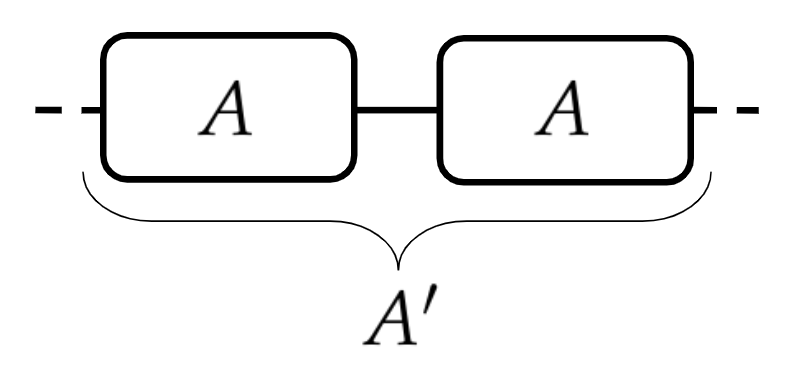
\includegraphics[scale=0.3]{Figures/wilson.png}
    \caption{Blocking scheme of Wilson's NRG method.}
    \label{fig:wilson}
\end{figure}

First of all, it is important to mention Wilson's numerical renormalization group (NRG) procedure, in which the CSR method is rooted. 

Let us consider a 1D-system made up by $N$ spins. The NRG method suggests to take two spins and consider a subspace of the corresponding Hilbert space $\mathcal{H}_2 \subset \mathcal{H}_1 \otimes \mathcal{H}_1$ of dimension $d_2 \leq d_1^2$; then, one adds a spin and consider the subset of the Hilbert space of three spins $\mathcal{H}_3 \subset \mathcal{H}_2 \otimes \mathcal{H}_1$ of dimension $d_3 \leq d_2d_1$, and so on until one arrives to consider the subset of Hilbert space $\mathcal{H}_N \subset \mathcal{H}_{N-1} \otimes \mathcal{H}_1$ with dimension $d_N \leq d_{N-1}d_1$. So, one can approximate the Hamiltonian with $P_NHP_N$, where the $P_N$ is the projector onto $\mathcal{H}_N$. If one chooses $d_N$ sufficiently small, one can diagonalize the Hamiltonian and find eigenvalues and eigenvectors. A good thing to do is fixing for all the dimensions $d_n$ the so-called \emph{bond dimension} such that 
\begin{equation*}
    d_n \leq D \quad \forall \quad n. 
\end{equation*}

We consider a one-dimensional spin chain;  the NRG method requires to break the chain into a set of identical blocks A (see fig.~\ref{fig:wilson}). So, one diagonalizes the Hamiltonian matrix $H_{AA}$ for two neighboring blocks $A$ and uses its lowest $m$ eigenstates (ordered by energy) to form a pseudo-unitary matrix $O$, employed to change the basis and make up the Hamiltonian $H_{A'}$ representing the block $A'$ twice as large (see fig.~\ref{fig:wilson}), in this way:
\begin{equation*}
    H_{A'} = OH_{AA}O^\dagger,
\end{equation*}
where $O$ is a $m\times n$ matrix (the rows of $O$ are the $m$ lowest eigenstates of $H_{AA}$) and $H_{AA}$ has dimension $n \times n$. This procedure has to be repeated using the new larger blocks $A'$ and the new effective Hamiltonian $H_{A'}$. 

\begin{figure}[H]
\centering
%\begin{subfigure}{6cm}
    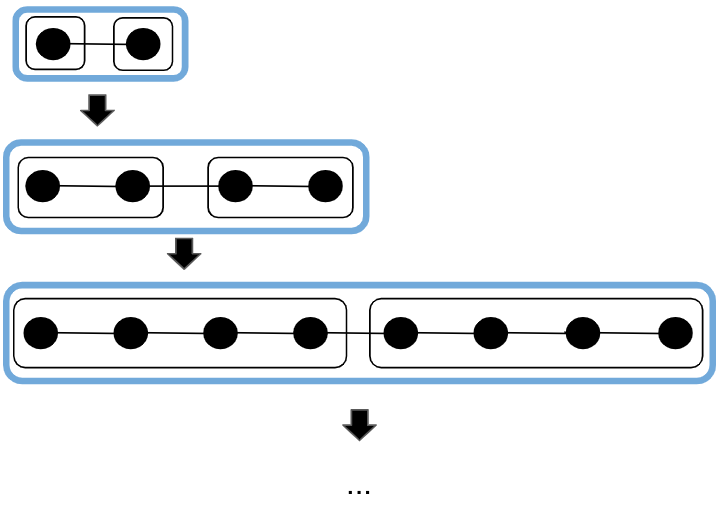
\includegraphics[width=0.5\linewidth]{Figures/blocks_wilson}
    \caption{Merging of the blocks in \\NRG procedure.}
    \label{fig:blocks_wilson}
%\end{subfigure}\quad
%\begin{subfigure}{6cm}
%    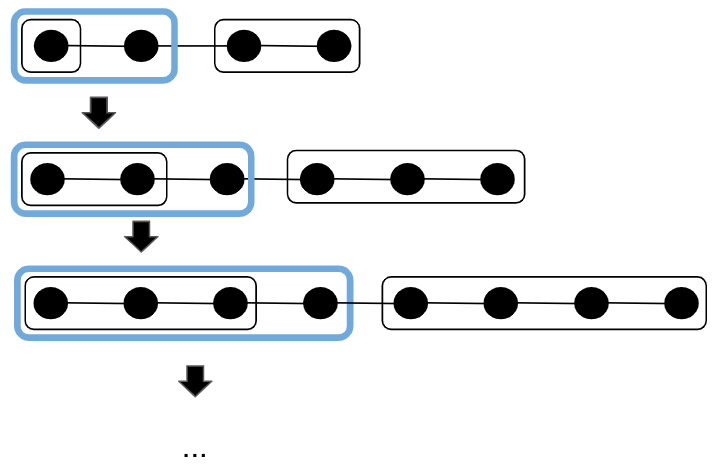
\includegraphics[width=\linewidth]{Figures/blocks_dmrg}
%    \caption{Merging of blocks (block+single site) in DMRG procedure.}
%    \label{fig:blocks_dmrg}
%\end{subfigure}
%\caption{Comparisons of blocking schemes of NRG and DMRG methods.}
%\label{fig:blocks}
\end{figure}

It is worth noting that the NRG method overlooks the connections between the blocks (see fig.~\ref{fig:blocks_wilson}), so it is a good method only in the limit that the links between the blocks vanish. This weak point has been studied and overcome by White in~\cite{s_white:dmrg} where he developed the DMRG method, that will be outlined in the following section.

The CSR method can be seen as a generalization of the NRG method, a development to the case of open systems. The name refers to the idea of selecting a \emph{corner} of the Hilbert space for a lattice system, using eigenvectors of the steady-state density matrix of smaller lattices.

Let us start considering two blocks of a quantum system consisting in a certain number $N$ of sites. The CSR approach is a recursive process that begins with the calculation of the steady-state density matrix of a small block (the first \emph{block} will be a single site, in the second iteration it will be a small lattice constituted of the two blocks emerged in the previous iteration, and so on); this calculation can be done studying the spectrum of the eigenvalue of the Liouvillian and taking the zero value, considered that
\begin{equation}
    \frac{d\rho}{dt} = \mathcal{L} \rho
\end{equation}
can be seen as an eigenvalue equation.

We now consider two spatially adjacent sites: the site A and the site B. We now call $\rho^{(A)}$ the steady-state density matrix of the first site and $\rho^{(B)}$ of the latter. In order to spatially merge these two sites, let us write $\rho^{(A)}$ and $\rho^{(B)}$ in terms of an orthonormal basis; if there is no degeneracy among eigevalues of $\rho^{(A)}$ and $\rho^{(B)}$, we can use the orthonormal basis formed by their eigenvectors. Instead, if there is degeneration, a Gram-Schmidt orthonormalization process can be used to obtain an orthonormal basis starting from the ensemble of eigenvectors.

In this way, we will have:
\begin{equation}
    \begin{split}
        \rho^{(A)} & = \sum_r p_r^{(A)}\ket{\phi_r^{(A)}}\bra{\phi_r^{(A)}}, \\
        \rho^{(B)} & = \sum_{r'} p_{r'}^{(B)}\ket{\phi_{r'}^{(B)}}\bra{\phi_{r'}^{(B)}},
    \end{split}
\end{equation}
where
\begin{equation*}
    \begin{split}
        p_r^{(A)} \geq 0 \quad \forall r \quad &\textrm{and} \quad p_{r'}^{(B)} \geq 0 \quad\forall r', \\
        \sum_{r} p_r^{(A)} = 1 \quad &\textrm{ and } \quad \sum_{r'} p_{r'}^{(B)} = 1.
    \end{split}
\end{equation*}
The steady-state density matrix of the \emph{merged block} constituted of the block A and the block B will be the following:
\begin{align}
\label{rhoAUB}
    \rho^{(AUB)} &= \rho^{(A)} \otimes \rho^{(B)} = \\
    \label{rhoAUB_explicit}
    &= \sum_{r} \sum_{r'} p_r^{(A)}p_{r'}^{(B)}\ket{\phi_r^{(A)}}\ket{\phi_{r'}^{(B)}} \otimes \bra{\phi_{r'}^{(B)}}\bra{\phi_{r}^{(A)}}
\end{align}
At this point, the CSR method suggests to delineate the \emph{corner-space}; for this purpose, we consider the $M$ most probable product states coming from~\ref{rhoAUB} of the form $\ket{\phi_{r}^{(A)}}\ket{\phi_{r'}^{(B)}}$, i.e. we rank the~\ref{rhoAUB_explicit} according to the joint probability $p_r^{(A)}p_{r'}^{(B)}$. The $M$ states form an orthonormal basis that generates a subspace
\begin{equation}
\label{basis_corner}
    \Bigl\{\ket{\phi_{r_1}^{(A)}}\ket{\phi_{r_1'}^{(B)}}, \ket{\phi_{r_2}^{(A)}}\ket{\phi_{r_2'}^{(B)}}, \dots, \ket{\phi_{r_M}^{(A)}}\ket{\phi_{r_M'}^{(B)}} \Bigl\},
\end{equation}
called \emph{corner-space}, with
\begin{equation*}
    p_r_1^{(A)}p_{r_1'}^{(B)} \geq p_r_2^{(A)}p_{r_2'}^{(B)} \geq \dots \geq p_r_M^{(A)}p_{r_M'}^{(B)}.
\end{equation*}
So, now it becomes necessary doing a change of basis to the new block $A \cup B$, that is:
\begin{equation}
    H' = \widetilde{O} H_{A\cup B} \widetilde{O}^\dagger,
\end{equation}
where $\widetilde{O}$ is a pseudo-unitary\footnote{The matrix $\widetilde{O}$ is called pseudo-unitary because it is not a square matrix.} $M\times N$ matrix, where $N$ is the dimension of $H_{A\cup B}$; $\widetilde{O}$ is formed by the $M$ eigenvectors of $\rho_{A\cup B}$ living in the corner-space. This density matrix can now be used to calculate the expectation values of any observable.

The more $M$ is large, the more the results are exact, because the basis~\ref{basis_corner} spans a larger part of the Hilbert space. Therefore, at this point the value of $M$ should be increased until the convergence is reached.

In the work of~\cite{PhysRevLett.115.080604} it has been proved that convergence can be achieved with a number of states $M$ much smaller than the dimension of the Hilbert space. In the present thesis, it will be shown that this method can not be used for the analysis of systems described by a model such as that under consideration in the present work.

%The resulting dimension of the space in which, from now on - re-iterating the procedure - the system will be studied, is made smaller.

\begin{figure}
    \centering
    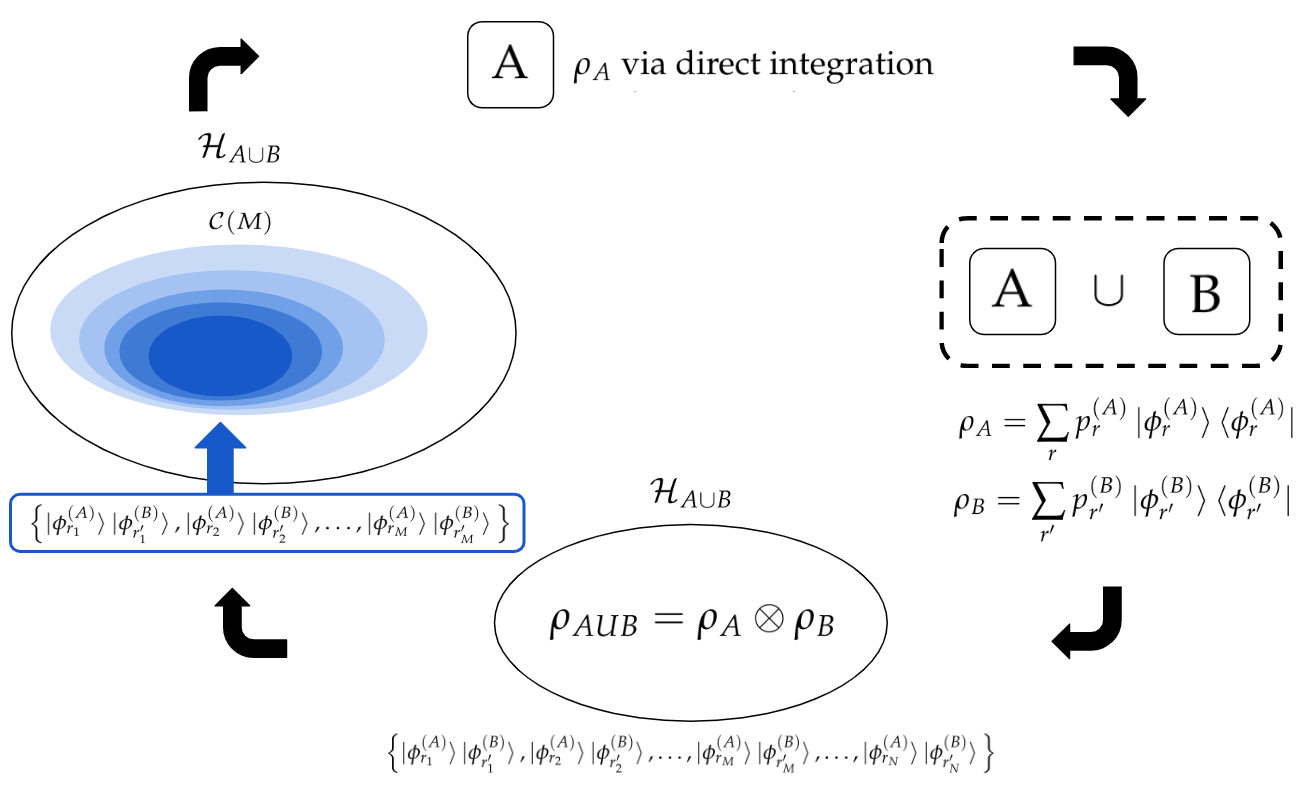
\includegraphics[scale=0.55]{Figures/csr_sketch}
    \caption{Sketch of the corner space renormalization method.}
    \label{fig:csr_sketch}
\end{figure}

\bigskip
In short, the algorithm is structured in the following stages, as sketched in fig.~\ref{fig:csr_sketch}:
\begin{description}
    \item[calculation] of the steady-state density matrix of a single block of the system;
    \item[merger] of two predetermined blocks;
    \item[expression] of the density matrix of the merged block in an orthonormal basis;
    \item[selection] of the M most probable states as a basis for the so-called \emph{corner-space};
    \item[increase] of the dimension M of the corner-space until the convergence of the observable is achieved.
\end{description}

A detailed description of the implementation of the algorithm can be seen in Appendix~\ref{AppendixA}.


%%%%%%%%%%%%%%%%%%%%%%%%%%%%%%%%%%%%%%%%%%%%%%%%%%%%%%%%%%%%%%%%%%%%%%%%%%%%%%%%%%%%%%%%%%%%%%%%%%%%%%%%%%%%%%%%%%%%%%%%%%%%%%%%%%%%%%%%%%%%%%%%%%%%%%%%%%%%%%%%%%%%%%%%%%%%%%%%%%%%%%%%%%%%%%%%
\section{The Matrix Product Density Operators (MPO) Method}
Finally, we analyze the \emph{matrix product density operators} (MPO) method.
This method is rooted in one of the first and most efficient numerical methods: the \emph{density matrix renormalization group} (DMRG)~\cite{s_white:dmrg, PhysRevB.48.10345, RevModPhys.77.259}.

Essentially, the DMRG is a generalization of Wilson's NRG method; the core of the method lies in the construction of the so-called \emph{superblock}, a block made up by 

the core of the DMRG method goes as follows: after the construction of a portion of the system, one enlarges it and in order to keep the size of the Hilbert space manageable, truncates its basis, keeping only the most relevant states, according to
\begin{equation*}
    \rho = \Tr_{E}()
\end{equation*}

\begin{figure}[H]
    \centering
    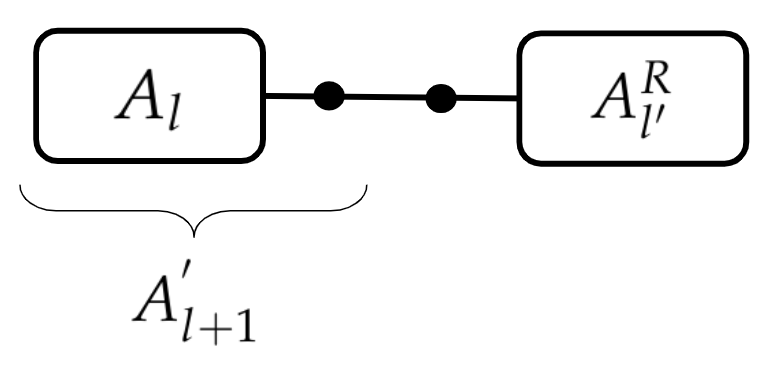
\includegraphics[scale=0.3]{Figures/DMRG_superblockSketch.png}
    \caption{Sketch of blocks configuration in DMRG method. The rectangles represent block of $l$ and $l'$ sites respectively, while the circles represent single sites.}
    \label{fig:DMRG_superblockSketch}
\end{figure}

The MPO method is the generalization of the \emph{matrix product states} (MPS) method \cite{SCHOLLWOCK201196}, which is useful in the description of (closed) quantum many-body systems. The essential idea~\cite{Cirac_2009} behind the MPS method lies in Wilson's renormalization group; in particular, 
So, let us consider the Hilbert space $\mathcal{H}_2$; we write an arbitrary orthonormal basis $\{\ket{\beta\}}_{\beta=1}^{d_2}$ as
\begin{equation*}
    \ket{\beta}_2 = \sum_{n_1, n_2}^d_1 B_\beta^{n_1, n_2} \ket{n_1}_1 \otimes \ket{n_2}_1,
\end{equation*}
where $B_\beta^{n_1, n_2}$ are the coefficients of the basis vectors in terms of the original basis vectors $\ket{n} \in \mathcal{H}_1$ and can be expressed as
\begin{equation*}
    B_\beta^{n_1, n_2} = \sum_{\alpha=1}^d_1 A[1]_\alpha^{n_1}A[2]_{\alpha,\beta}^{n_2},
\end{equation*}
where $A[1]_\alpha^{n_1} = \delta_{n1, \alpha}$ and $A[2]_{\alpha,\beta}^{n_2} = B_\beta^{\alpha, n_2}_\beta$. So, we can now write any orthonormal basis in $\mathcal{H}_3$ in terms of $\ket{\beta}_2\otimes \ket{\ket{n_3}}$ and go on iteratively. After M steps, we have:
\begin{equation*}
    \ket{\beta}_M = \sum_{\alpha=1}^{d_{M-1}}\sum_{n_M=1}^{d_1} A[M]_{\alpha,\beta}^{n_M}\ket{\alpha}_{M-1}\otimes\ket{n_M}_1,
\end{equation*}
that is, substituting recursively the definition of $\ket{\alpha}_m$:
\begin{equation*}
    \ket{\beta}_N = \sum_{n_1,\dots,n_N=1}^{d_1} (A_1^{n_1}A_2^{n_2}\dots A_N^{n_N})_\beta \ket{n_1,\dots,n_N},
\end{equation*}
i.e.
\begin{equation}
\label{mps_general}
    \ket{\psi_{MPS}} = \sum_{n_1,\dots,n_N=1}^{d_1} A_1^{n_1}A_2^{n_2}\dots A_N^{n_N} \ket{n_1,\dots,n_N}.
\end{equation}
Because of the form of , this vectors are called \emph{matrix product states} (MPS). %\textcolor{red}{FIGURA DAL CIRAC2009 PAGINA 16}

For periodic boundary conditions the form of the~\ref{mps_general} is obtained performing the trace over their product~\cite{SCHOLLWOCK201196, PhysRevLett.93.207204}:
\begin{equation}
    \ket{\psi_{MPS}} = \sum_{n_1,\dots,n_N=1}^{d} \Tr(A_1^{n_1}A_2^{n_2}\dots A_N^{n_N}) \ket{n_1,\dots,n_N}.
\end{equation}
One should note that the total number of parameters turns out to be $N \times d \times D^2$, i.e. it is linear in $N$.

The matrix product \emph{density operators} (MPO) extend the MPS from pure to mixed states, following the idea explained, for example, in~\cite{PhysRevLett.93.207204}. The physical index is now doubled, as illustrated in fig.~\ref{fig:tensor_network}%\textcolor{red}{FIGURA}:
\begin{equation}
\label{eqn:mpdo}
    \rho_{MPO} = \sum_{i_1, \dots ,i_N = 1}^{d} \sum_{j_1, \dots ,j_N = 1}^{d} \Tr\Bigl(A_1^{i_1,j_1} \dots A_N^{i_N,j_N}\Bigl) \ket{i_1, \dots ,i_N}\bra{j_1, \dots ,j_N}.
\end{equation}
The $A^{[k]i_k,j_k}$ are $D^2 \times D^2$ tensors that can be decomposed in this way:
\begin{equation*}
    A_k^{i,j} = \sum_{a = 1}^{d_k} M_k^{i,a} \otimes (M_k^{j,a})^*.
\end{equation*}

Another way of considering the expression~\ref{eqn:mpdo} is the graphical notation to represent a tensor $A^{[k] i,j}$ sketched in figure~\ref{fig:tensor_network}. Here, every tensor is represented by a square with 4 legs: there are two of them for the bonds with the neighbours, the other two for the physical indices (the "bras" and "kets"). 

\begin{figure}[H]
    \centering
    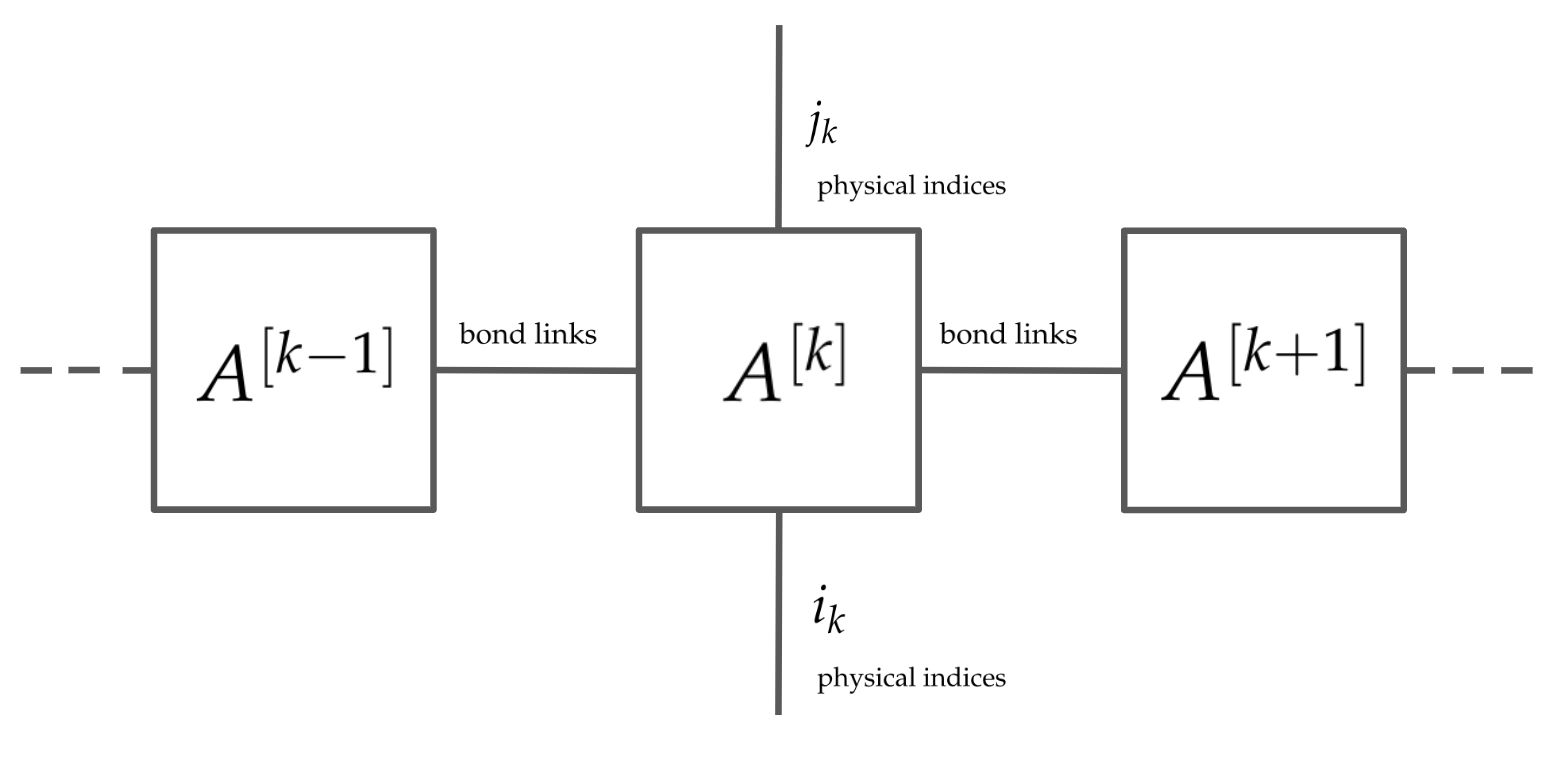
\includegraphics[scale=0.30]{Figures/tensor_network.png}
    \caption{Graphical notation of tensors in a 1D system.}
    \label{fig:tensor_network}
\end{figure}

As regards dynamics, the long-time limit of eq.~\ref{eqn:lindblad_eqn} can be reached using a MPO ansatz for the density matrix. The steady-state solution $\rho$ is found using an algorithm based on the \emph{time evolution block decimation} (TEBD)~\cite{PhysRevLett.91.147902} scheme adapted to open systems. It is useful, for instance, to efficiently compute time-dependent properties of 1D closed quantum many-body systems as done in~\cite{PhysRevLett.93.040502}. 

Here, we can briefly see how it works~\cite{jin_biella_ross} in the case of open many-body systems in the MPO formalism. 

First of all, let us consider the~\ref{eqn:mpdo}: repeated single-value decomposition of the tensor $C_{i_1,\dots, i_N; j_1,\dots, j_N}$ can lead to
\begin{equation*}
\label{mpo_ansatz}
\begin{split}
    \rho_{MPO} = \sum_{i_1, \dots ,i_N = 1}^{d}\quad \sum_{j_1, \dots ,j_N = 1}^{d}\quad \sum_{\alpha_1,\dots, \alpha_{N-1} = 1}^\chi &(\Gamma_{1, \alpha_1}^{[1]i_1, j_1}\lambda_{\alpha_1}^{[1]})(\Gamma_{\alpha_1, \alpha_2}^{[2]i_, j_2}\lambda_{\alpha_2}^{[2]}) \dots \\  \times &(\lambda_{\alpha_{N-1}}^{[N-1]}\Gamma_{N, \alpha_{N-1}}^{[N]i_N, j_N}) ||i_1, \dots ,i_N, j_1, \dots ,j_N\rangle\rangle.
    \end{split}
\end{equation*}
where the superoperator formalism is been used in order to write the superket \\$||i_1, \dots ,i_N, j_1, \dots ,j_N\rangle\rangle$. The bond-link dimension $\chi$ can be kept under a threshold by discounting the smallest single values; moreover, it is proportional to the amount of quantum correlation between the system sites that can be embedded in $\rho_{MPO}$.

%As shown in~\cite{Prosen_2009, PhysRevLett.93.207205}, $\hat{\mathcal{L}}$ %can be decomposed into terms that involve two contiguous sites, as
%\begin{equation}
%    \hat{\mathcal{L}}[\rho] = \sum_l \hat{\mathcal{L}}_{l,l+1}[\rho].
%\end{equation}
Formally, the solution of~\ref{eqn:lindblad_eqn} can be written as
\begin{equation}
\label{eqn:lindblad_dinamics}
    \rho(t) = e^{\hat{\mathcal{L}}t}\rho(0).
\end{equation}
Following the Vidal's work~\cite{PhysRevLett.93.040502}, the liouvillian superoperator $\hat{\mathcal{L}}$ can be decomposed in this way:
\begin{equation}
    \hat{\mathcal{L}} = \hat{F} + \hat{G},
\end{equation}
where
\begin{equation}
    \begin{split}
        \hat{F} &\equiv \sum_{\text{even } l} \hat{F}^{[l]} \equiv \sum_{\text{even } l} (\hat{\mathcal{L}}_2^{l, l+1}) \\
        \hat{G} &\equiv \sum_{\text{odd } l} \hat{G}^{[l]} \equiv \sum_{\text{odd } l} (\hat{\mathcal{L}}_2^{l, l+1}), \\
        l  &= 1, \dots N-1
    \end{split}
\end{equation}
having considered a Liouvillian made of arbitrary nearest-neighbouring interaction terms.

For every small time step $\tau > 0$, the Trotter-Suzuki expansion of order $p$ for $\exp{(\hat{\mathcal{L}} t)}$ reads:
\begin{equation*}
    e^{\hat{\mathcal{L}}t} = e^{(\hat{F}+ \hat{G})t} = \prod_k \exp{(\alpha_k\hat{\mathcal{L}}_1\tau)}\dots\exp{(\beta_k\hat{\mathcal{L}}_N\tau)} + \mathcal{O}(\tau^p),
\end{equation*}
with $p$ depending on the required accuracy.

%\textcolor{red}{VEDI PRESENTAZIONE GARNET CHAN - RIVEDERE \\ AGGIUNGERE FORMALISMO SUPEROPERATORIALE}

%\noindent\rule[0.5ex]{\linewidth}{1pt}
%\noindent\rule[0.5ex]{\linewidth}{1pt}

%One can express a MPDO in terms of a pure state MPS using the \emph{purification}~\cite{nielsen_chuang} technique. The essential idea is to consider an auxiliary system with a Hilbert space of dimension $d_k$ and, after choosing an orthonormal basis $\ket{i_k, a_k}$, to write the corresponding MPS state as
%\begin{equation}
%    \ket{\psi} = \sum_{i_1,\dots,i_N} \sum_{a_1, \dots, a_N} Tr\Bigl(\prod_{k=1}^N B_k^{i_k, a_k}\Bigl) \ket{i_1a_1, \dots, i_Na_N}.
%\end{equation}
%and eventually the MPDO $\rho$ is obtained tracing over the indices referred to the auxiliary system $a_k$:
%\begin{equation}
%    \rho = Tr_a(\ket{\psi}\bra{\psi});
%\end{equation}
%this density matrix can be used to compute the expectation values of observables.
\chapter*{Conclusions}
\addcontentsline{toc}{chapter}{Conclusions}

\label{Conclusions}

In the presented work, we have focused on the study of strong correlated quantum systems driven on the edge by quantum baths. %steady-state system

One could wonder why it would be interesting study such a system: the answer comes from the breakthroughs in  experimental methods, e.g. in the field of ultracold atoms and QED cavities, the platforms that make it possible to reproduce Hamiltonian models not analyzeable otherwise and consequently to understand complex quantum-physical phenomena. 

In the work developed in the previous pages, we have concentrated upon a model, in particular: an anisotropic XYZ Heisenberg spin-1/2 chain driven far from equilibrium with a pair of dissipators acting on the edge of the chain only.

%Lindblad equation
In such a system two kind of dynamics compete: the Hamiltonian one and the dissipative one. We have studied the steady-state to which the system tends while these two dynamics act; in this state, we have analyzed three observables under different regimes of dissipation and of Hamiltonian evolution: magnetization profile, two-point correlation function, spin current.

With regard to 

%AGGIUNGI ANCHE IL FATTO CHE HAI USATO METODI NUMERICI

%perché è interessante studiare sistemi dissipativi, interesse generale
%cosa abbiamo trovato
%ci siamo concentrati sullo studio dei sist quant fort corr in cui metto dissipaz ai bordi e vado a vedere sullo stato stazionario che sistema si forma, che caratteristiche ha: questo è interessante perché ci sono piattaforme sperimentali che permettono di studiare...
%nella tesi abbiamo scoperto che prendendo un heisenberg xyz si generano profili etc etc
%1-2 pagine

%----------------------------------------------------------------------------------------
%	THESIS CONTENT - APPENDICES
%----------------------------------------------------------------------------------------

\appendix % Cue to tell LaTeX that the following "chapters" are Appendices

% Include the appendices of the thesis as separate files from the Appendices folder
% Uncomment the lines as you write the Appendices

\chapter{The Corner-Space Renormalization Algorithm} % Main appendix title

\label{AppendixA}
%\chapter{Additional Plots}
\label{appendix_supplemental}

In this section we show some useful plots in appendix of the study of magnetization profile, two-point correlation function and spin transport in the model analyzed.

\section{Supplemental Plots on Magnetization Profile}

As anticipated in section~\ref{sec:magn_profile}, along x and y direction the magnetization profile is trivial, because the dissipators act only along z direction. This is displayed in fig.~\ref{fig:comparisonSigmaXYZ} for a 8-sites chain with $J_z = 1$ and $\gamma = 1$, but it has been found the same result also for other parametrizations of the system.

\begin{figure}[H]
    \centering
    \captionsetup{width=1.\linewidth}
    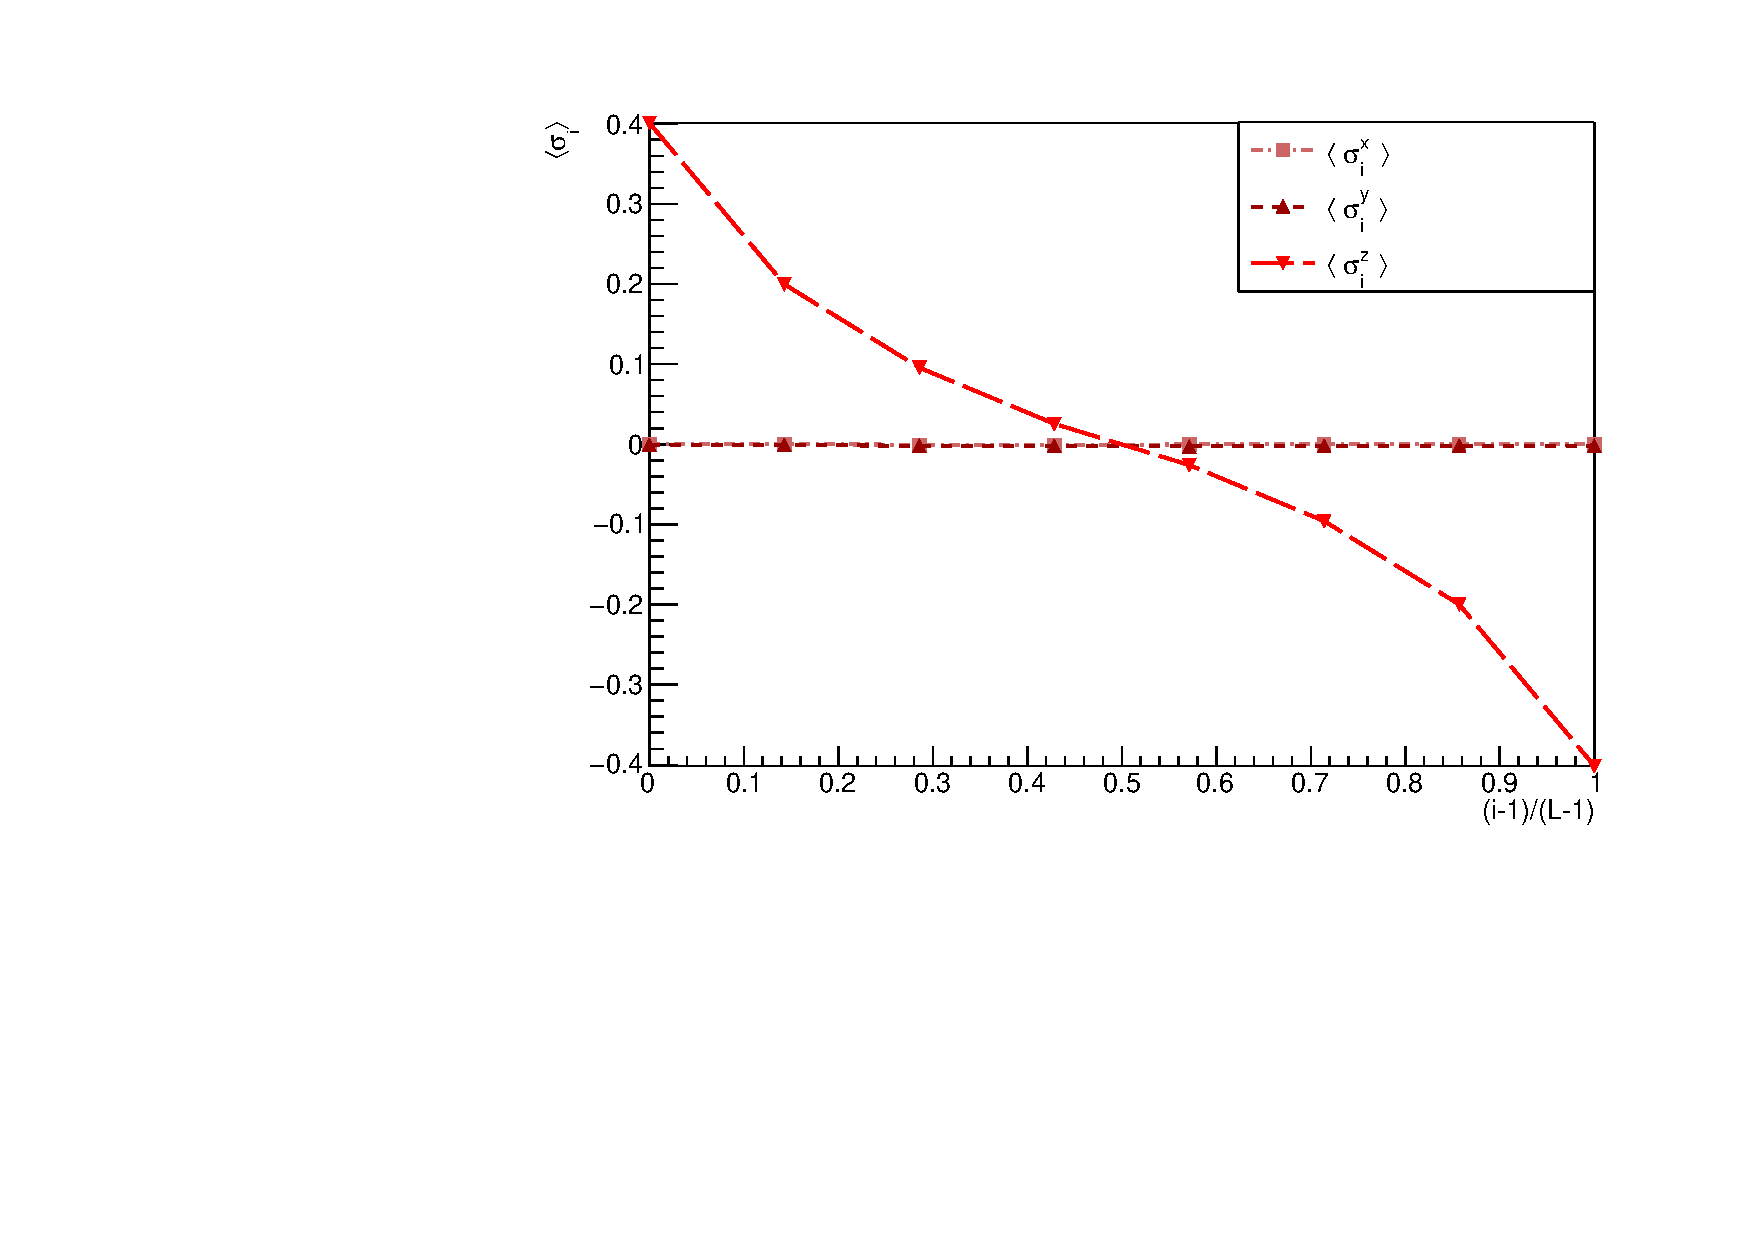
\includegraphics[scale=0.6]{Figures/comparisonSigmaXYZ.pdf}
    \caption{Magnetization profile along the x, y and z spin direction, for a 8-sites chain with $J_z = 1$ and $\gamma = 1$.}
    \label{fig:comparisonSigmaXYZ}
\end{figure}

The magnetization along z direction of every spin of the chain, increases with $\gamma$ following an exponential trend. This is confirmed also by the study of the gradient $\nabla \sigma^z$, the fit of which shows a dependence as the following:
\begin{equation*}
    \nabla \sigma^z (\gamma) = - p_0 + p_1 e^{-p_2\gamma},
\end{equation*}
as displayed in fig.~\ref{fig:FIT_12sites_gradLM34VSgamma}, for a 16-sites chain, for which the gradient between the third and the forth spins has been analyzed.
\begin{figure}[H]
    \centering
    \captionsetup{width=1.\linewidth}
    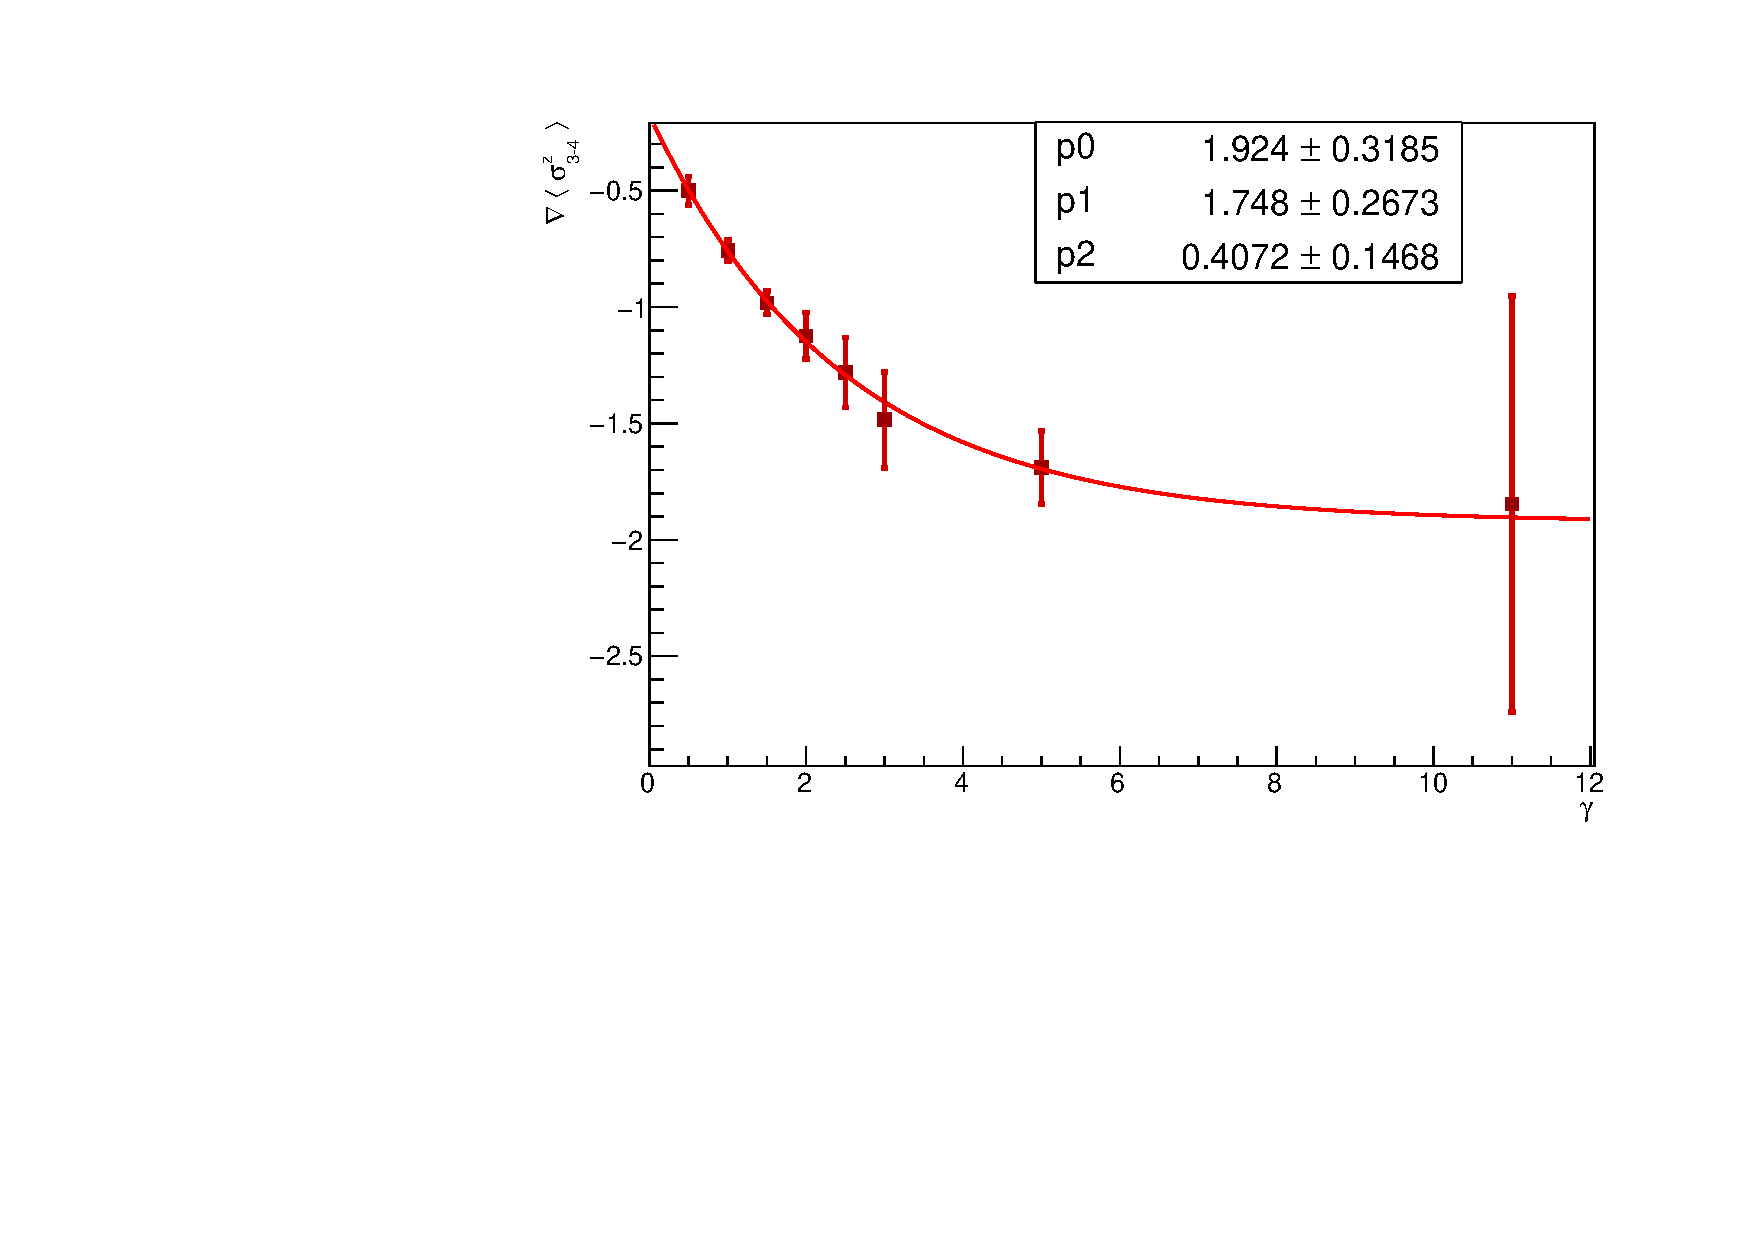
\includegraphics[scale=0.6]{Figures/16sites_gradLM_3and4VSgamma.pdf}
    \caption{Profile of the gradient between the third and the forth site of a 16-sites chain versus $\gamma$. The fit shows an exponential profile.}
    \label{fig:FIT_12sites_gradLM34VSgamma}
\end{figure}

Another feature mentioned in section~\ref{sec:magn_profile}, is the fact that while $\gamma$ grows, the expectation value of $\sigma^z$ tends asymptotically to a limit value, that depends on the site under consideration. In section~\ref{sec:magn_profile}, the coefficient that controls this rate has been named $p_1$. In fig.~\ref{fig:16sites_p1VSsiteIndex} we see that $p_1$ has a linear dependence on the site position.

%il primo punto è un effetto dovuto al bordo, dove risente della presenza del bagno c'è il dissipatore; il resto è costante. Da 5 in poi i punti sono molto vicini a zero, non li plttaimo perché abbiamo valori piccoli e non riusciamo ad avere uns tima accurata di p. Nel primo sito c'è un offset prob dovuto alla pres del bagno, perchè il sistem anon è omogeneo. Negli altri siti è praticamente costante. 

\begin{figure}[H]
    \centering
    \captionsetup{width=1.\linewidth}
    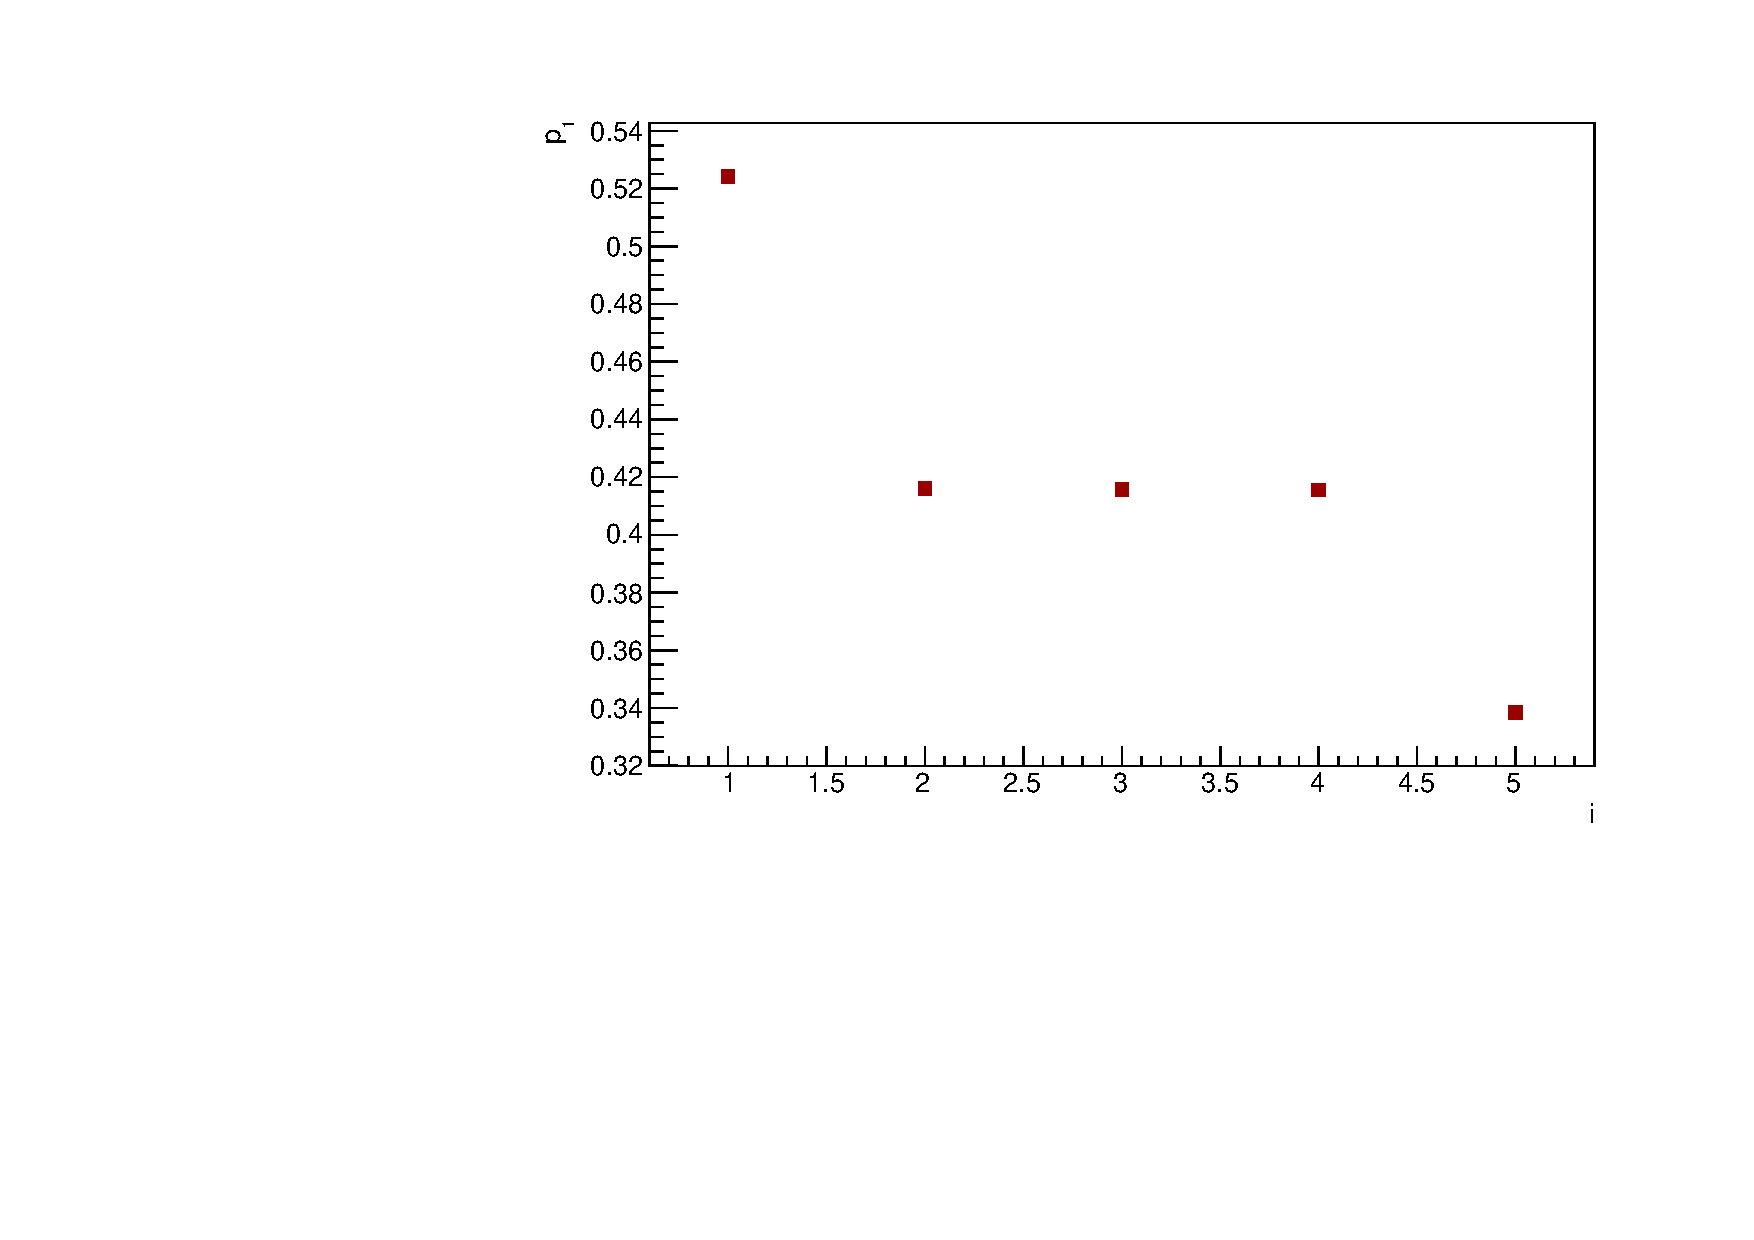
\includegraphics[scale=0.6]{Figures/16sites_p1VSsiteIndex.pdf}
    \caption{Growth rate coefficient $p_1$ versus site index. Beyond the fifth site the profile is no longer exponential because of the zero magnetization plateau.}
    \label{fig:16sites_p1VSsiteIndex}
\end{figure}

\section{Supplemental Plots on Correlations}
We have seen that the bulk correlation function, defined in section~\ref{sec:2P_correlationFunction}, has an exponential profile, with a decay rate coefficient $p_1$ that depends on $\gamma$, with a dependence shown in fig~\ref{fig:CFBulkCONN_p1vsGamma}. The non-monotonic profile is probably due to the competion between Hamiltonian dynamics and dissipative dynamics.

\begin{figure}[H]
    \centering
    \captionsetup{width=1.\linewidth}
    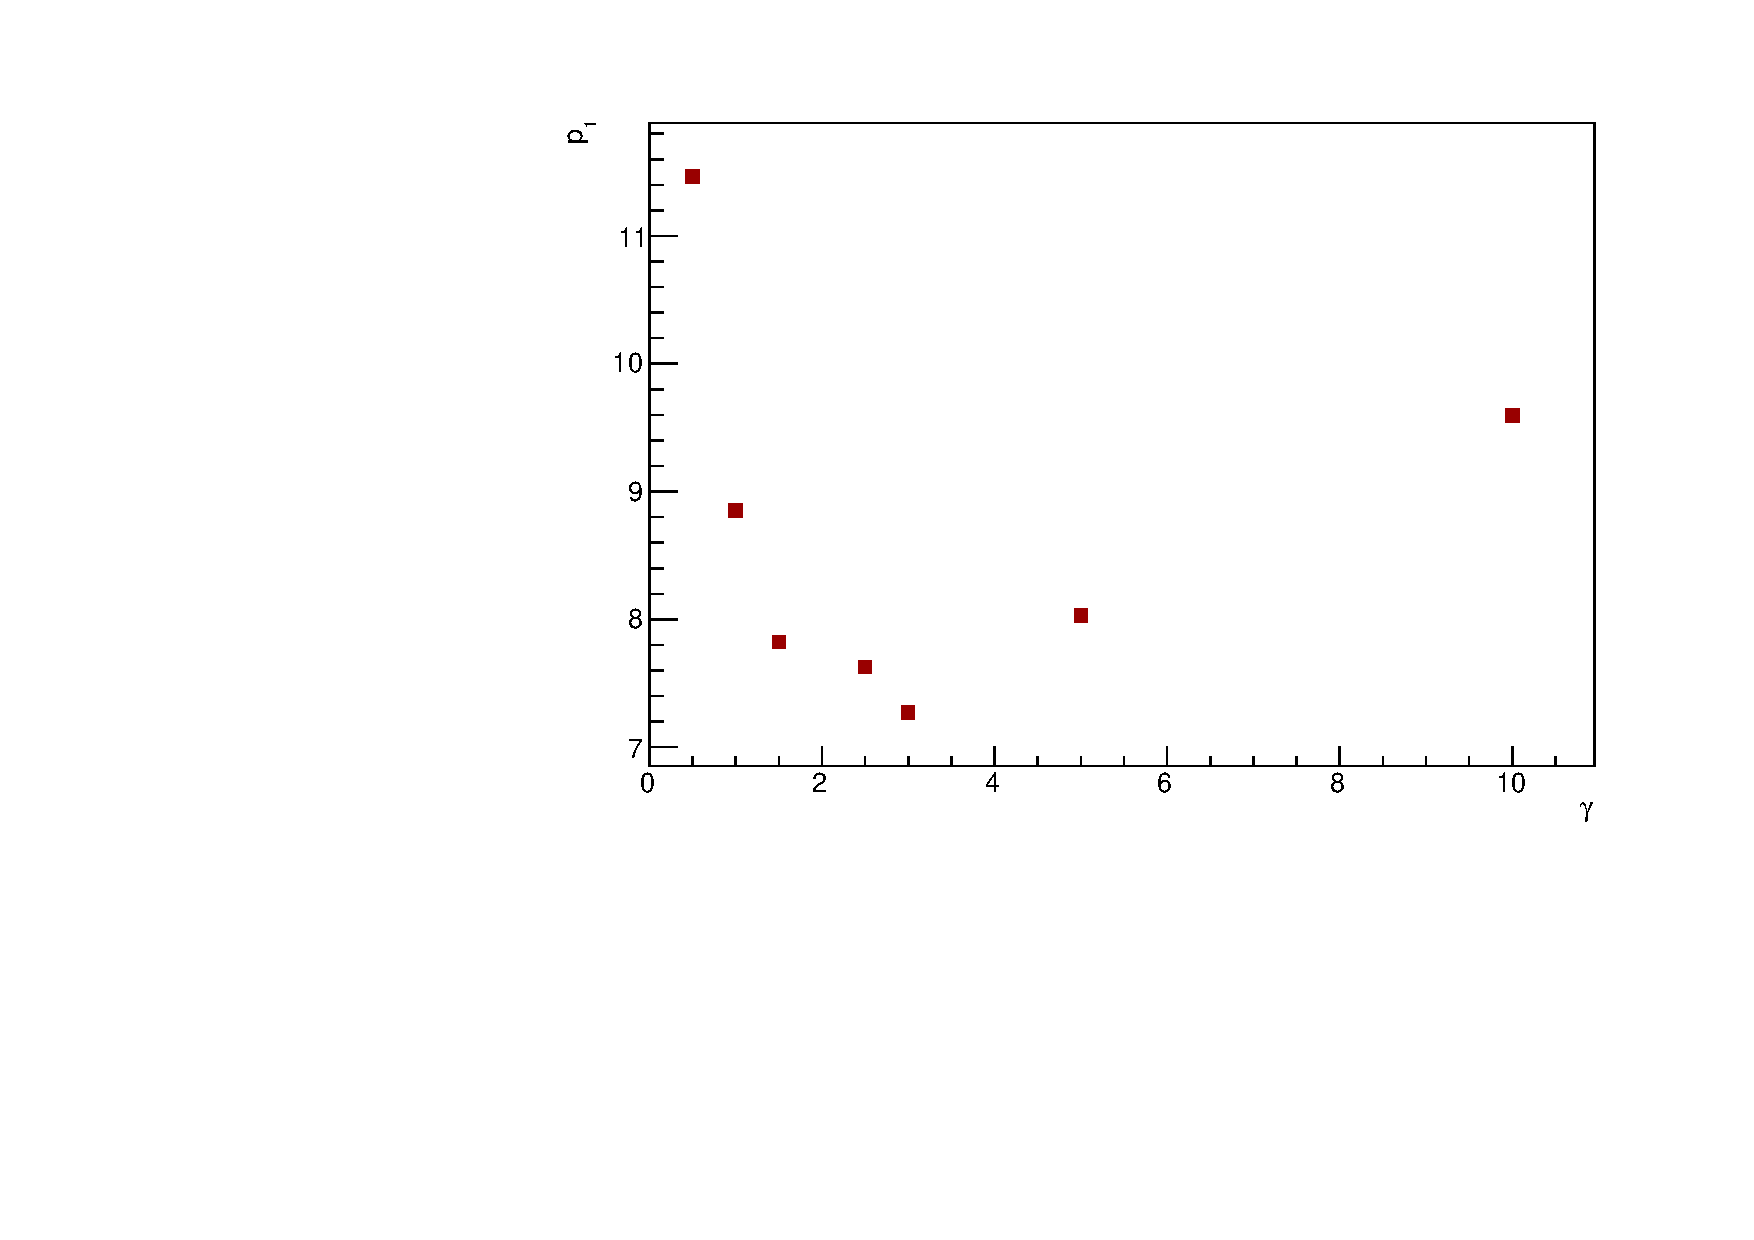
\includegraphics[scale=0.6]{Figures/CFBulkCONN_p1vsGamma.pdf}
    \caption{Rate coefficient $p_1$ versus $\gamma$. The trend is non-monotonic, due to the competition between the Hamiltonian and dissipative dynamics.}
    \label{fig:CFBulkCONN_p1vsGamma}
\end{figure}

\section{Supplemental Plots on Spin Transport}
As we have seen in section~\ref{spin_curr}, the spin current depends on $J_z$. The spin current between the first two spins and the last two spins of the chain is shown in fig.~\ref{fig:SpinCurrVSJz1st} and in fig.~\ref{fig:SpinCurrVSJzLth} respectively. 

It is clear that the peak values of spin current are independent of $J_z$ while $J_z < 0.9$; from $J_z \geq 1$, it rapidly decays to zero. This is probably due to the fact that if the Hamiltonian dynamics gets a predominant role over the dissipative dynamics,the system does not detect any driven effect, so it reacts like there was no dissipative forces.

\begin{figure}[H]
    \centering
    \captionsetup{width=1.\linewidth}
    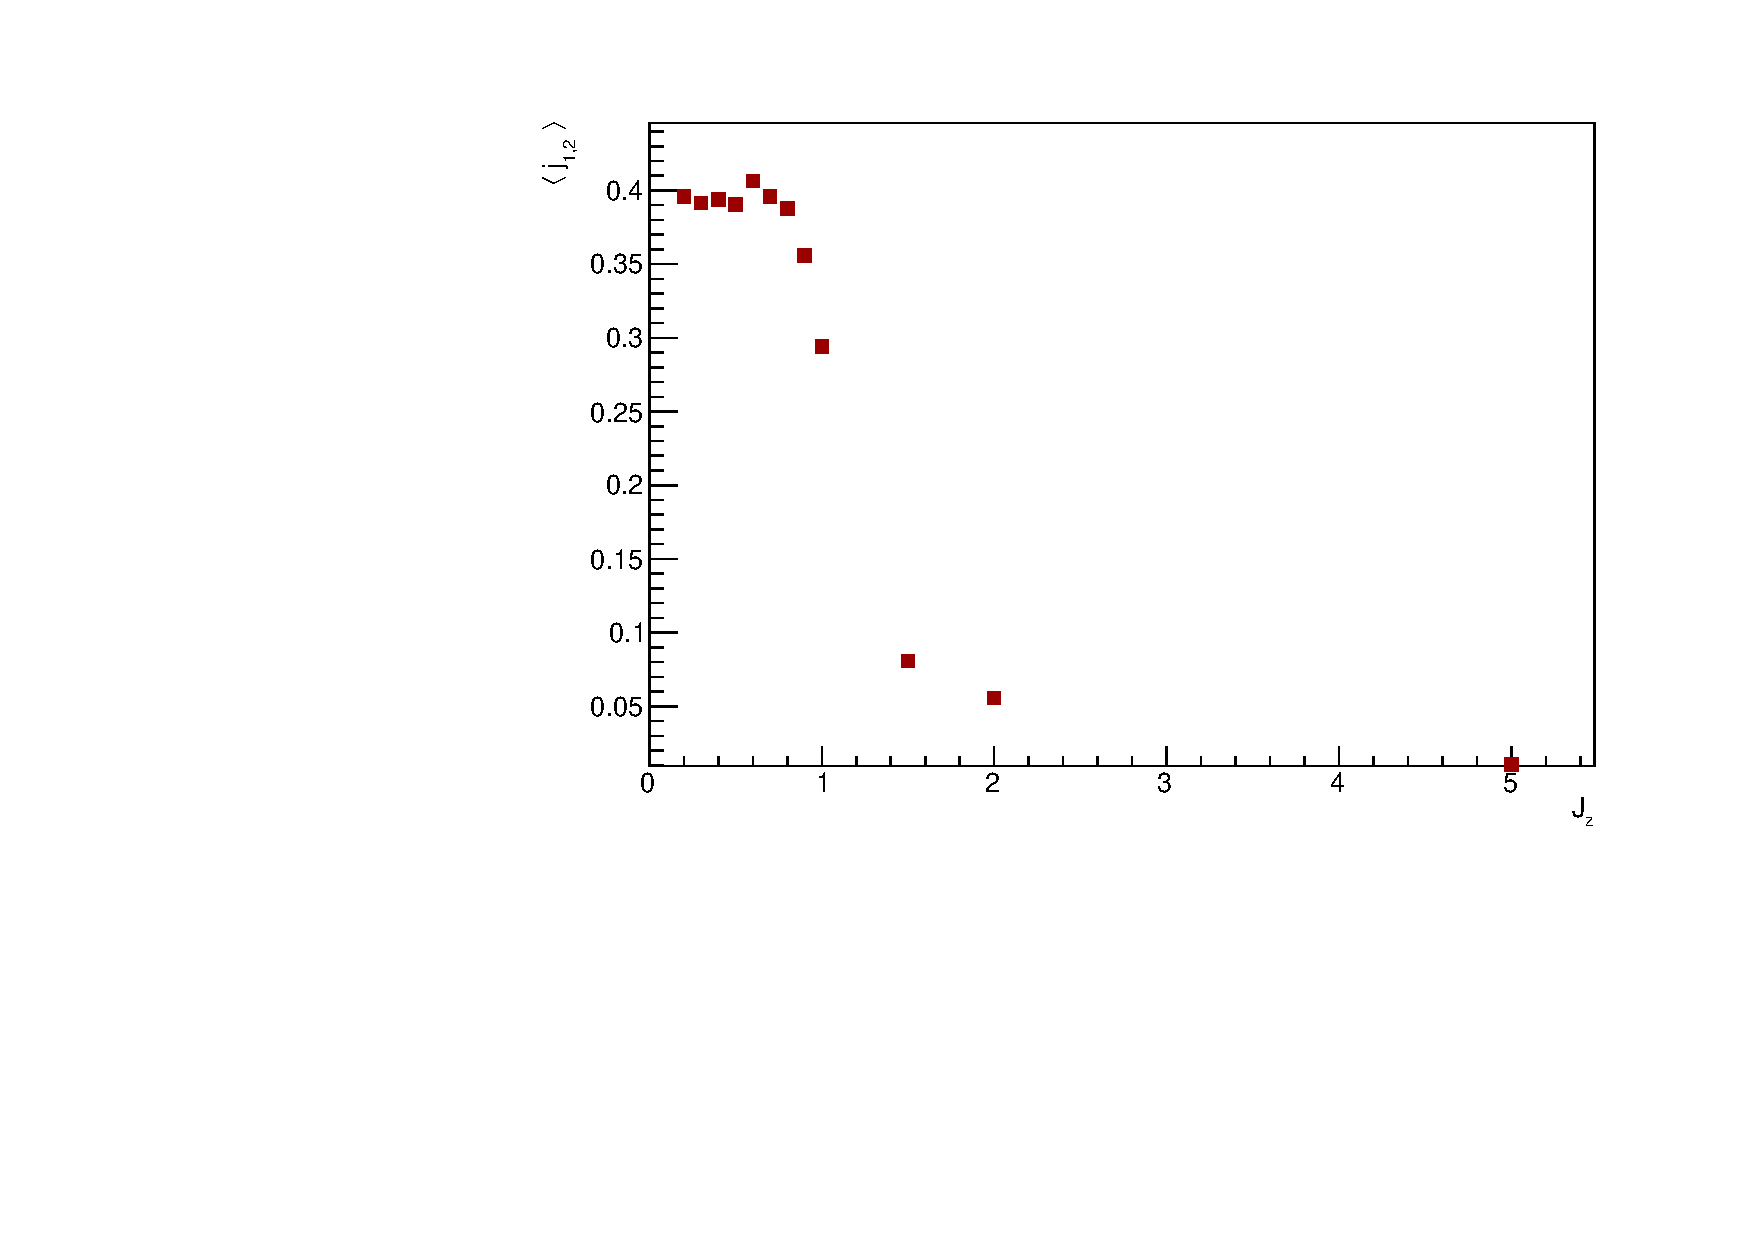
\includegraphics[scale=0.6]{Figures/SpinCurrVSJz1st.pdf}
    \caption{Spin current between the first two spins of a 16-sites chain, with $\gamma=1$ versus several values of $J_z$. Errors have been estimated as explained in section~\ref{sec:MPO_errors}.}
    \label{fig:SpinCurrVSJz1st}
\end{figure}

\begin{figure}[H]
    \centering
    \captionsetup{width=1.\linewidth}
    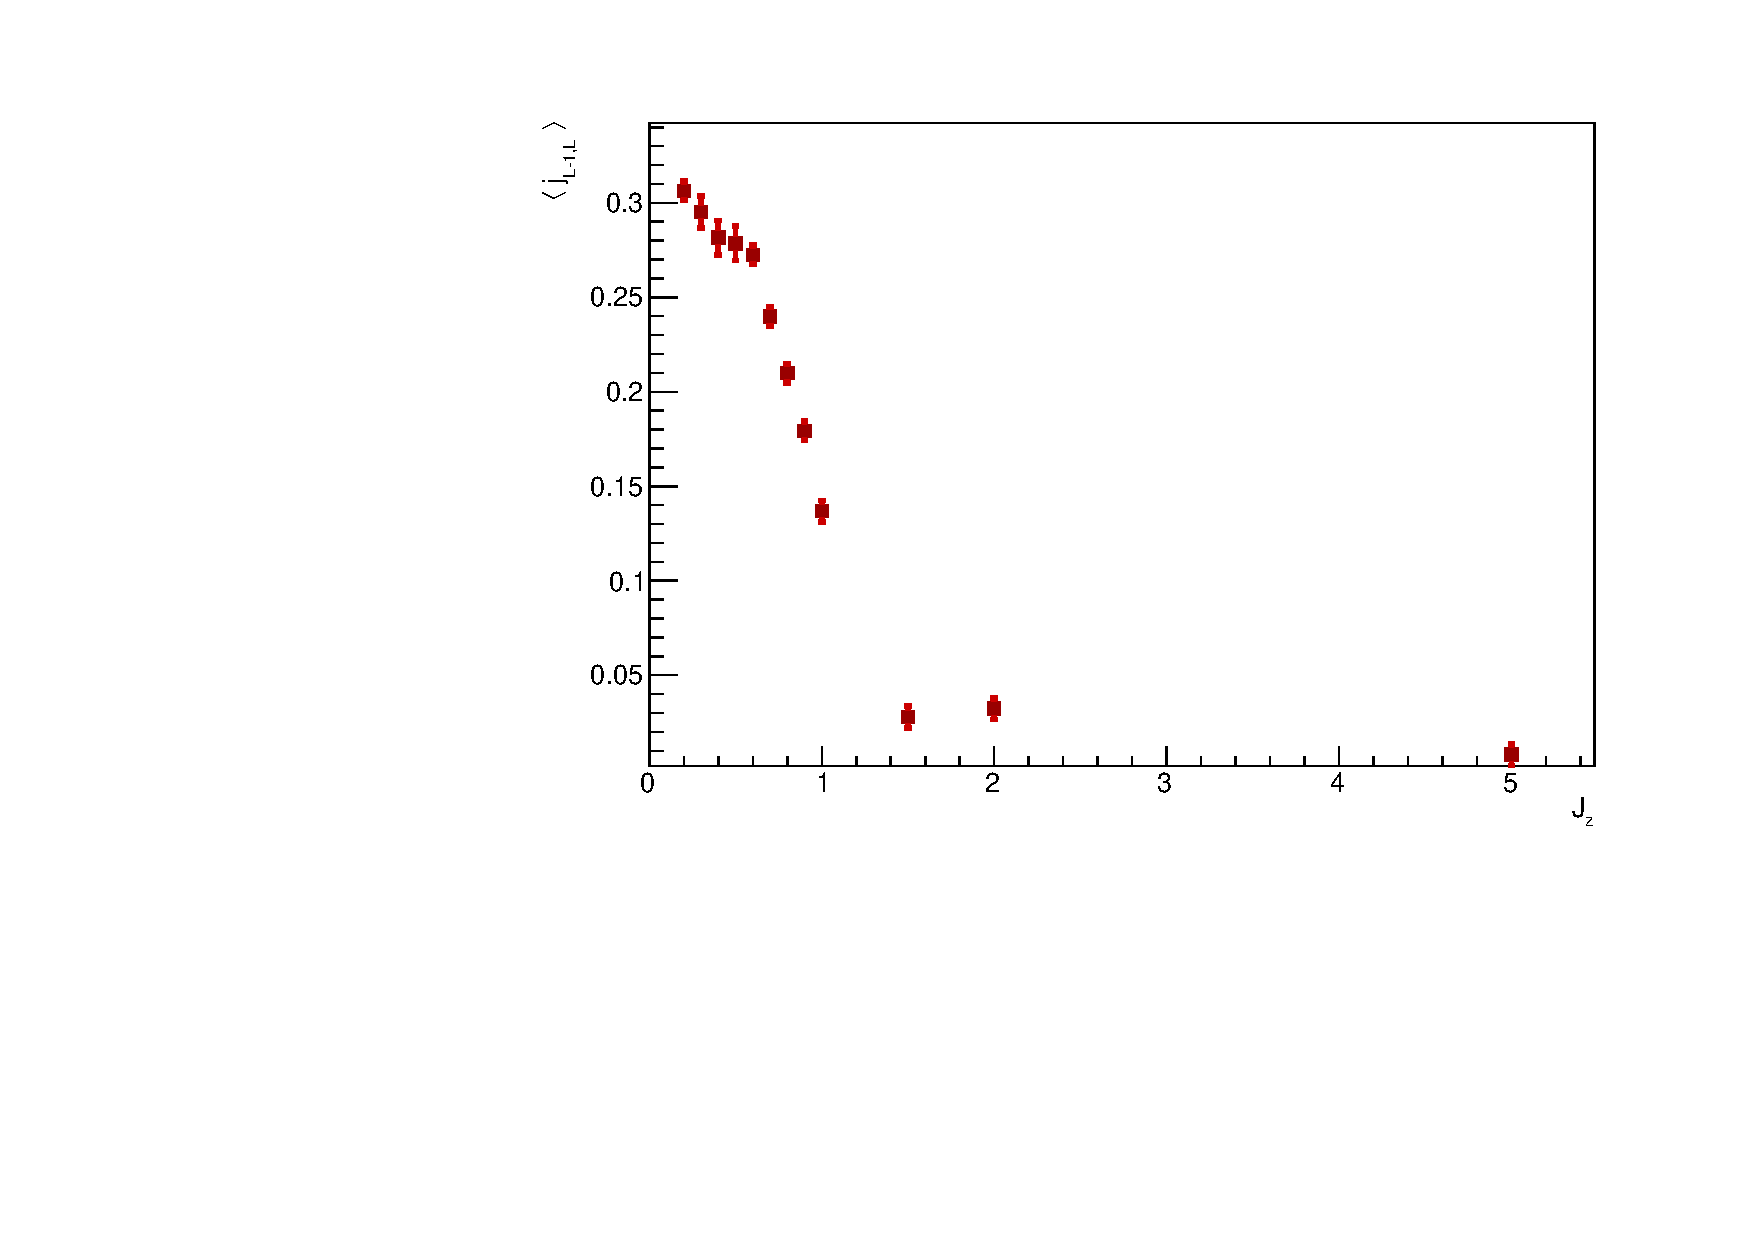
\includegraphics[scale=0.6]{Figures/SpinCurrVSJzLth.pdf}
    \caption{Spin current between the last two spins of a 16-sites chain, with $\gamma=1$ versus several values of $J_z$. In contrast to $j_{1,2}$, in this case there is a decreasing profile even for $J_z < 0.9$. This could be true or it be due to the difficulty on reaching convergence for this values of $J_z$. The numerical errors are displayed by the red error bars in the plot and they have been estimated as explained in section~\ref{sec:MPO_errors}.}
    \label{fig:SpinCurrVSJzLth}
\end{figure}
%\chapter{Lower Size Chains}
\label{AppendixC}

%----------------------------------------------------------------------------------------
%	BIBLIOGRAPHY
%----------------------------------------------------------------------------------------

\nocite{*}
\printbibliography[heading=bibintoc]

%----------------------------------------------------------------------------------------

%----------------------------------------------------------------------------------------
%	ACKNOWLEDGEMENTS
%----------------------------------------------------------------------------------------

\begin{acknowledgements}
\addchaptertocentry{\acknowledgementname} % Add the acknowledgements to the table of contents
The acknowledgments and the people to thank go here, don't forget to include your project advisor\ldots
\end{acknowledgements}

\end{document}  
